\documentclass[11pt,twocolumn]{article}
\usepackage[margin=0.8in]{geometry}                % See geometry.pdf to learn the layout options. There are lots.
\geometry{letterpaper}                   % ... or a4paper or a5paper or ... 
%\geometry{landscape}                % Activate for for rotated page geometry
%\usepackage[parfill]{parskip}    % Activate to begin paragraphs with an empty line rather than an indent
\usepackage{color}
\definecolor{myblue}{rgb}{0.0, 0.0, 0.85}
\usepackage[breaklinks=true, colorlinks=true, linkcolor=red, urlcolor=myblue, citecolor=black]{hyperref}
\urlstyle{rm}
\usepackage{amsmath}
\usepackage{mathptmx}
\usepackage{graphicx}
\usepackage{amssymb}
\usepackage{epstopdf}
\usepackage{sidecap}
\usepackage{authblk}
\usepackage{booktabs}
\usepackage[font=small,labelfont=bf]{caption}
\DeclareGraphicsRule{.tif}{png}{.png}{`convert #1 `dirname #1`/`basename #1 .tif`.png}
\usepackage{enumitem}
\setlist[itemize]{noitemsep}
\setlist[enumerate]{noitemsep}

\usepackage{draftwatermark}
\SetWatermarkText{DRAFT}
\SetWatermarkScale{1}
\SetWatermarkColor[gray]{0.85}

\def\bfr{\bf\color{red}}
\def\geohub{{\tt geohub}}
\def\Count{count}
\def\ntracts{40}
\def\nprof{9}
\def\nvol{31}
\def\resp{respectively}
\def\nch{715}
\def\nh{956\pm94}
\def\dh{10\%\pm9\%}
\def\nce{389}
\def\ne{556\pm83}
\def\de{15\%\pm12\%}

%\raggedbottom

\title{\bf
	Results of the 2021 Greater Hollywood Volunteer Homeless Count
	}
\author[1,2,3,$\dagger$]{Louis Abramson}
\author[4]{Brian Kohan}
\author[1,5]{Jackie Vorhauer}
\author[1,6]{Heather Carmichael}
\author[1,7]{Helen Eigenberg}
\author[1,8]{Stephen Fiechter}
\author[1]{David Gordon}
\author[9]{Courtney Kanagi}
\author[1,10]{Emily Uyeda Kantrim}
\author[9]{Guido Merkens}
\author[1,10]{Arnali Ray}
\author[5]{Elyse Schwartz}
\author[1,5]{Douglas Walker}
\author[1]{Kerry Morrison}
\affil[1]{\it \small Hollywood 4WRD Homelessness Coalition, 6255 Sunset Blvd, Ste 150, Los Angeles, CA 90028}
\affil[2]{\it Central Hollywood Neighborhood Council, PO Box 93907, Los Angeles, CA 90093}
\affil[3]{\it Carnegie Observatories, 813 Santa Barbara St, Pasadena, CA 91101}
\affil[4]{\it SELAH Neighborhood Homelessness Coalition, 2658 Griffith Park Blvd, Unit 194, Los Angeles, CA 90039}
\affil[5]{\it The Center in Hollywood, 6636 Selma Ave, Los Angeles, CA 90028}
\affil[6]{\it My Friend's Place, 5850 Hollywood Blvd, Los Angeles, CA 90028}
\affil[7]{\it Hang Out Do Good, 153 S Norton Ave, Los Angeles, CA 90004}
\affil[8]{\it People Assisting The Homeless, 340 N Madison Ave, Los Angeles, CA 90004}
\affil[9]{\it The Hollywood Partnership, 6562 Hollywood Blvd, Los Angeles, CA 90028}
\affil[10]{\it Mid City West Community Council, 644 N Fuller Ave, PMB 7059, Los Angeles, CA 90036}
\affil[$\dagger$]{Corresponding author; \href{mailto:labramson.chnc@gmail.com}{labramson.chnc@gmail.com}}

\date{\vspace{-1em}Draft: \today}                                           % Activate to display a given date or no date

\begin{document}
\maketitle

\begin{abstract}

Data from February 25, 2021 censuses of Hollywood and East Hollywood show that 
unsheltered homelessness has fallen by $\dh$ and $\de$, \resp, in those communities
compared to the 2020 LAHSA Count (90\% CI). A 30\% drop in individuals seen on the street 
drives this change, reducing the number of identified persons and dwellings in about a third of 
census tracts. The unsheltered population is thus likely to have declined even 
if average dwelling occupancies are updated. Nevertheless, 28\% of tracts saw at least a doubling 
of tents and makeshift structures. This enhanced visual salience---combined with COVID-related 
sanitation and social service disruptions---would support perceptions that conditions worsened 
over the past year despite the potential success of initiatives to bring and keep Angelenos indoors. 
Coordinated Entry System data will reveal whether homelessness has declined in general, or 
merely Greater Hollywood's unsheltered portion.

%This enhanced visual salience of unsheltered living---combined with 
%COVID-related disruptions to health and social services and increases drug-related 
%deaths---would support perceptions that conditions worsened for those remaining on the street
%despite the success of interventions aimed at bringing or keeping Angelenos indoors. 


\end{abstract}

\section{Context}
\label{sec:intro}

The Los Angeles Homelessness Services Authority (LAHSA) conducts an annual Point In Time (PIT) 
census of Los Angeles County's unhoused population. These data inform programmatic funding levels, 
educate residents, undergird legislation, and shape the practices of professional and volunteer 
service providers. 

As the official assessment of the scope of one of our most pressing humanitarian issues, the LAHSA Count 
is invaluable. Due to disruptions from COVID-19, however, the unsheltered portion of the 2021 count was 
cancelled. Since 70\% of unhoused residents of the City of LA (``LA'') were unsheltered in 2020, without 
additional efforts, this cancellation will substantially erode our understanding of homelessness following 
an unprecedented year of economic disruption and government intervention---both of which may have 
significantly affected the number of unhoused Angelenos.

Greater Hollywood is an epicenter of the homelessness crisis. According to the 2020 Count, the 
Hollywood and East Hollywood Communities were home to 2203 unhoused residents, 1714 of whom 
(78\%) were unsheltered. This figure corresponds to roughly 
\href{https://www.lahsa.org/data?id=45-2020-homeless-count-by-community-city}
{5\% of LA's homeless population} in an area with 3.5\% of its total population.\footnote{
\url{https://geomap.ffiec.gov/FFIECGeocMap/GeocodeMap1.aspx}; assumes 4M total Angelenos.} 
In some places, 1-in-25 Hollywood residents are unhoused compared to 1-in-100 citywide.

While the above statistics are tragic, Hollywood is also home to large and increasingly robust
coalitions of service providers, business leaders, residents, and governmental entities dedicated to 
humanely housing everyone in their community. Given the capacity of the above organizations and 
the importance of the annual PIT count in educating residents, funders, and legislators, Hollywood 
proceeded as a collective to conduct a grassroots PIT \Count\ on Thursday, February 25, 2021.

This document details the methodology and findings of that \Count. 
Section \ref{sec:procedure} describes the volunteer training, data acquisition, 
and analysis protocols. Section \ref{sec:results} presents estimates of the unsheltered 
populations in Hollywood and East Hollywood, contextualizes them in terms of the 2020 
LAHSA PIT results and those communities' total populations, and presents cross-checks. 
Section \ref{sec:discussion} provides interpretation and highlights areas where quantitive findings 
may drive qualitative impressions as to the ``felt'' state of the crisis. Section \ref{sec:summary} 
summarizes. The Appendix provides additional information, including tract-level tallies and 
population inferences. All data are available at {\bfr website}.

\section{Methods}
\label{sec:procedure}
%
%The \Count\ took place on 25 February 2021 circa at 7.00 PM. This timing corresponds to one month 
%after and four hours before the official event would have occurred. Beyond those choices, our program 
%adhered as closely as possible to the official LAHSA 2020 PIT data collection and analysis protocols. 
%
%The \Count\ was launched from The Center at Blessed Sacrament (``The Center''), a major service 
%provider in Hollywood, at 6636 Selma Ave. All volunteer teams reported and returned to this 
%location as they would to a LAHSA community hub in past years, but, as COVID precautions, 
%training was performed remotely in the week preceding the count and volunteers never left their 
%vehicles.

\subsection{Data Acquisition}
\label{sec:acquisition}

The \Count\ was based out of {\it The Center in Hollywood} (``The Center''), a major service 
provider in Hollywood. All volunteers reported and returned to this location as they would a LAHSA 
community hub in the past.\footnote{Except for those counting tract 1919.02; see Section \ref{sec:191902}.} 
Unlike previous PIT counts, however, training was performed offsite, volunteers never left their vehicles, 
and all surveying occurred before 10:00 PM.

The \Count\ covered the \ntracts\ US Census tracts constituting the LAHSA-defined 
\href{https://www.lahsa.org/data?id=45-2020-homeless-count-by-community-city}{Hollywood 
and East Hollywood Communities} (22 and 18 tracts, \resp). It did not recognize census 
tract ``splits''---e.g., ``1905.10a''---which modified of the definition of Hollywood to include 
all of tract 1905.10 and East Hollywood to include all of tract 1913.01. Since 2016, split 1905.10b 
has never hosted more than 7 unsheltered people; 1913.01a never more than 15. As such,
these modifications do not significantly affect community-level results.
%Sections \ref{sec:results} and \ref{sec:discussion} discuss community-level results with 
%tract-level tallies provided in the Appendix. Results for Greater Hollywood are not directly comparable 
%to any official service geography but are available upon request. 
Figure \ref{fig:map} shows the \Count\ footprint.

All tracts were vetted by outreach professionals from The Center prior to assignment. Tracts 
deemed especially challenging---e.g., due to their proximity to freeway onramps/peripheries---were 
reserved for professional counting teams. Vetting produced \nprof\ such tracts, which were surveyed 
by personnel from The Center and Covenant House circa 3:00 PM on 25 Feb. All but one of the remaining 
tracts were surveyed by volunteer vehicle-based teams and beginning at 7:00 PM. The final volunteer tract 
was surveyed on 16 March (Section \ref{sec:191902}).

With the exception of one tract in East Hollywood, teams were restricted to one or the other community, 
making the community-level results nearly independent. Cross-comparisons therefore serve as data 
quality indicators (Section \ref{sec:crossChecks}). Table \ref{tbl:tractStats} records which tracts were 
surveyed by which kind of team. 

Thirty-two volunteer teams participated in the \Count, which was limited to existing ``pods'' of two 
to three people to minimize the possibility of COVID transmission. 
%Singlet volunteers were admitted 
%but remained on-site to assist with traffic control and material distribution. 
All participants wore 
personal protective equipment and maintained social distancing when appropriate.

\begin{figure*}[t!]
	\centering
	\includegraphics[width=0.8\linewidth]{totalPopMap}
	\includegraphics[width=0.8\linewidth]{diffMap}
	\caption{The 2021 volunteer \Count\ covered the LAHSA-recognized Hollywood and East 
			Hollywood Communities. The former spans Laurel Canyon at Franklin to Western
			at Melrose. The latter spans Western at Hollywood to Hoover at Temple. 
			{\it Top:} inferred 2021 unsheltered population (darker is higher). 
			{\it Bottom:} inferred change from 2020 (red$+$, blue$-$). The tracts with the 
			largest gain (1912.01) and loss (1927.00) from 2020 are highlighted
			in both panels.}
	\label{fig:map}	
\end{figure*}

Counting followed 2020 LAHSA PIT protocols to the greatest extent possible. Each volunteer team 
comprised at least a driver and a counter and was assigned two tracts. Three-person teams 
included a navigator, as well. If present, the navigator directed the driver while the counter tallied 
individuals/dwellings. In two-person teams, the counter doubled as the navigator. Training 
emphasized techniques aimed at reducing counters' cognitive loads to minimize errors (e.g., 
covering interior streets in a serpentine pattern before circling the tract border). Teams were 
instructed to count both sides of interior streets but only interior sides of border streets 
as described in the official 2020 PIT training materials.

All teams were deployed by roughly 7:30 PM and returned by 9:55 PM.

Upon arriving at The Center, organizers gave each team a clipboard containing two tract maps,
two tally sheets, and a 1-page training summary with a contact number for field issues.

The tally sheets were the data acquisition tool. These contained separate columns for each of the 
nine categories of unsheltered individuals/dwellings recognized in the 2020 LAHSA PIT count: 
\begin{enumerate}
	\item adults (ages $\geq$25);
	\item transition age youths (``TAY,'' 18--24);
	\item unaccompanied minors;
	\item families (at least one adult with at least one minor); 
	\item cars;
	\item vans;
	\item RVs;
	\item tents;
	\item makeshift structures.
\end{enumerate}
Dwellings---items (5) to (9)---are treated specially in the analysis and hereafter 
may be referred to as ``CVRTM.'' Adults+TAY may also be combined into 
``Persons'' (P). No families or unaccompanied minors were identified.\footnote{
One potential unaccompanied minor was reported in tract 1912.01 but could not be confirmed by outreach
personnel dispatched to that location. One potential family was also reported dwelling in a van in
tract 1899.05 but could also not be confirmed. These categories' upper limits capture this 
uncertainty (3 each at 95\% confidence), but their raw counts are set to zero.} See Appendix for examples
of the above documents.

Upon returning, counters verbally read their results to organizers who entered them into a google 
form. Organizers verbally confirmed the counts before submitting the form and recovering the
paper tally sheets.
%Volunteer email addresses were also retained for follow-up. 

Once all materials were collected, organizers cross-checked the electronic records---a
google sheet generated by the form responses---with the paper tallies and identified any 
uncounted areas. None requiring follow-up were found. Disagreements between electronic 
and paper references were corrected to the paper tally. 
%All data are available at {\bfr website}.

Given turnout, every volunteer tract was assigned to at least two teams. Four tracts were 
counted in triplicate. Beyond increasing the \Count's accuracy, repeat measurements 
enhance our understanding of errors (Sections \ref{sec:dupes}) and provide robustness: one 
tally was uninterpretable, leaving only the result from the second team.

All told, the data comprise 38 pair-wise volunteer measurements, one unique volunteer measurement, 
and nine unique professional assessments. The latter account for $\sim$20\% of tracts in both communities 
and roughly 40\% of identified individuals and dwellings. Year-on-year trends are consistent between
volunteer- and professional-counted tracts (Section \ref{sec:crossChecks}). 
%---29 duplicates + 
%4 triplicates (=8 additional pairs)---
%The largest increase was observed by volunteers, the largest
%decrease by professionals.%; both tracts are located in E.~Hollywood.

\subsubsection{Tract 1919.02}
\label{sec:191902}

Tract 1919.02 escaped assignment on the night of the \Count. This omission was recognized 15 March
and the area independently surveyed by experienced volunteers at 6:00 AM (Abramson) and 
8:15 PM (Eigenberg) the next day. Despite the 19-day delay, we include these data to conform the 
2021 PIT results to LAHSA-defined geographies. While \href{https://selahnhc.org}
{SELAH} tract monitoring suggests counts are stable on $\sim$month timescales, no conclusions
change if this tract is excluded.% counts are consistent to <1sigma in total and per category.

\begin{table}[t!]
\caption{2021 Greater Hollywood PIT Count Summary}
\resizebox{\linewidth}{!}{%
\begin{tabular}{cccccc}
\toprule
Tract & Community & Counter$^{\rm a}$ & Passes$^{\rm b}$ & Median Est. & 90\% CI \\ 
 & & & & [people] & [people] \\ \cmidrule{1-6}
1898.00 & Hollywood & Vol & 3 & 6 & 0--15 \\
1899.02 & Hollywood & Vol & 3 & 18 & 12--24 \\
1899.03 & Hollywood & Vol & 2 & 0 & 0--12 \\
1899.04 & Hollywood & Vol & 2 & 18 & 11--25 \\
1899.05 & Hollywood & Vol & 2 & 19 & 9--30 \\
1901.00 & Hollywood & Vol & 2 & 88 & 75--102 \\
1902.01 & Hollywood & Vol & 2 & 21 & 13--29 \\
1902.02 & Hollywood & Vol & 2 & 30 & 20--40 \\
1903.01 & Hollywood & Pro & 1 & 74 & 54--96 \\
1905.10 & Hollywood & Pro & 1 & 34 & 22--46 \\
1905.20 & E.~Hollywood & Vol & 2 & 12 & 6--18 \\
1907.00 & Hollywood & Vol & 2 & 110 & 93--127 \\
1908.01 & Hollywood & Vol & 2 & 63 & 50--76 \\
1908.02 & Hollywood & Pro & 1 & 71 & 54--90 \\
1909.01 & Hollywood & Pro & 1 & 55 & 39--71 \\
1909.02 & Hollywood & Vol & 3 & 6 & 0--17 \\
1910.00 & Hollywood & Pro & 1 & 169 & 140--201 \\
1911.10 & E.~Hollywood & Vol & 2 & 9 & 2--15 \\
1911.20 & E.~Hollywood & Pro & 1 & 66 & 48--85 \\
1912.01 & E.~Hollywood & Vol & 2 & 55 & 44--68 \\
1912.03 & E.~Hollywood & Vol & 2 & 26 & 14--38 \\
1912.04 & E.~Hollywood & Vol & 2 & 6 & 0--16 \\
1913.01 & E.~Hollywood & Vol & 2 & 31 & 22--42 \\
1913.02 & E.~Hollywood & Vol & 2 & 23 & 15--30 \\
1914.10 & E.~Hollywood & Vol & 2 & 20 & 13--28 \\
1914.20 & E.~Hollywood & Vol & 2 & 24 & 16--32 \\
1915.00 & E.~Hollywood & Vol & 2 & 29 & 21--38 \\
1916.10 & E.~Hollywood & Pro & 1 & 48 & 31--68 \\
1916.20 & E.~Hollywood & Pro & 1 & 17 & 6--30 \\
1917.10 & Hollywood & Vol & 2 & 21 & 14--29 \\
1917.20 & Hollywood & Vol & 3 & 21 & 12--31 \\
1918.10 & Hollywood & Vol & 2 & 24 & 14--34 \\
1918.20 & Hollywood & Vol & 2 & 16 & 10--23 \\
1919.01 & Hollywood & Vol & 2 & 60 & 49--72 \\
1919.02$^{\rm c}$  & Hollywood & Vol & 2 & 19 & 13--27 \\
1925.10 & E.~Hollywood & Vol & 2 & 12 & 4--21 \\
1925.20 & E.~Hollywood & Vol & 1$^{\rm d}$ & 14 & 1--28 \\
1926.10 & E.~Hollywood & Vol & 2 & 7 & 1--14 \\
1926.20 & E.~Hollywood & Vol & 2 & 18 & 9--26 \\
1927.00 & E.~Hollywood & Pro & 1 & 129 & 96--167\\
\cmidrule{1-6}
{\bf All} & & & {\bf 74} & {\bf 1510} & {\bf 1361--1679}\\ 
\bottomrule
\end{tabular}
}
\caption*{$^{\rm a}$Volunteer vs.~professional surveyor; $^{\rm b}$no.~counting teams; 
		$^{\rm c}$ surveyed 16 March; $^{\rm d}$one tally rejected during quality control.}
\label{tbl:tractStats}
\end{table}

\subsubsection{Volunteer Training}
\label{sec:training}

Teams underwent mandatory, $\sim$30 minute Zoom-based training sessions before arriving 
for the \Count. Each participant was also required to watch the official 
\href{https://www.youtube.com/watch?v=ul94Jt6l68w}{2020 LAHSA PIT training video}.% and sign participation waivers.

The training covered the motivation for the \Count, an overview of the survey geography, team roles, 
and examples of unhoused dwellings. Except for people standing next to tents---as described 
in the 2020 LAHSA video---volunteers were instructed to count CVRTM and individuals separately 
and not to estimate how many people might live in or be associated with a specific dwelling. 
This ensured that results could be analyzed as a function of the CVRTM weights, which may change 
with future information.% (see Section \ref{sec:analysis}).

The training primed volunteers only with min/max estimates of tract-level individual+dwelling 
counts (``0--120'') and the likelihood of encountering unaccompanied minors or families (``very unlikely'')
or TAY (``some tracts, especially in Hollywood''). These statements were informed by the 2020 
LAHSA PIT results. No other prior was established. The training presentation is available 
\href{https://drive.google.com/file/d/1xFrtU26yjPuiUv9KHZ3Uj2_sAoT1ClGo/view?usp=sharing}{here}.

\subsection{Data Analysis}
\label{sec:analysis}

The data form a $9\times75$ array containing each team's tract-level tallies for each unhoused 
individual/dwelling class. The population inference entails averaging duplicate tract counts and 
weighting CVRTM by their mean occupancies. We produce 10,000 realizations of this inference 
incorporating random perturbations of the counts and weights based on their 
errors (see below). The final product is a $9\times10000\times\ntracts$ array that may be split and 
summed to provide aggregate, tract, or category-level population estimates and uncertainties.

Our baseline result assumes the 
\href{https://www.lahsa.org/documents?id=4635-usc-2018-2020-multipliers-and-estimates-overview.pdf}
{2020 SPA4/CD13 CVRTM weights} underpinning the 2020 LAHSA 
\href{https://www.lahsa.org/documents?id=4686-2020-greater-los-angeles-city-community-homelessness-report-service-planning-area-4.pdf}{Community Summaries}. We recognize that these weights may have changed since they were last
defined and encourage robust efforts to reassess them. However, at least one survey of tent-dwellers in Hollywood 
suggests that the tent weight has remained stable. Section \ref{sec:comp} reviews the impact of adopting
the other CVRTM choices in Table \ref{tbl:weights}; none significantly affects our findings.
%COVID-related activities such as tent  distribution efforts may have changed

%While an estimate of the underlying population, uncertainties in each visual count and weight 
%must be accounted for to understand how confident one can be that that estimate corresponds to
%the truth. We accomplish this by using Monte Carlo integration to construct the full probability
%distribution functions (PDFs) for the number of unsheltered people of each class in each tract.

% {\it These results will
%correspond to the most likely values for the respective quantities in any geography.} However,
%three uncertainties---one small and two large---complicate the interpretation of those sums. 
%We discuss these in Section \ref{sec:discussion}, but account for them as best we can using 
%Monte Carlo techniques to construct the full underlying probability distribution functions (PDFs) 
%for each class in each tract.
%
%All results discussed below derive from 10,000 Monte Carlo realizations of Item (5), above.
%

\subsubsection{Monte Carlo Population Inferences}
\label{sec:mc}

We wish to infer the true unsheltered population in Hollywood and East Hollywood as of 25 February. 
We do so by constructing probability density functions (PDFs) describing the likelihood of encountering 
a given number of unsheltered people in those communities as constrained by our PIT data. 
To accomplish this, we model three known uncertainties: (1) errors in the visual tallies, (2) deviations 
of the CVRTM weights from their quoted means, and (3) the intrinsic background rate of persons/dwellings
in areas where none were actually sighted. Items (1) and (3) reflect how our PIT tally might change
if performed at a different time or by different teams. Item (2) reflects how the mean 
occupancy of CVRTM in our survey area might differ from that in the geography in which the weights 
were defined.

We model count and weight errors as independent random draws from Gaussian distributions with 
standard deviations of $\sqrt{n}$ and $\sigma$, \resp, where $n$ is the raw PIT tally and 
$\sigma$ is the standard error on the respective CVRTM weight, $w$. 
The $i$-th estimate of the true number, $N$, of people in the $j$-th unsheltered class in any 
tract is then: 
\begin{multline}\label{eq:monte}
	N_{i,j} = \left[n_{j} + \mathcal{G}_{i}(0,\sqrt{n_{j}})\right]\times\max[\mathcal{G}_{i}(w_{j}, \sigma_{j}),1],
\end{multline}
where $\mathcal{G}(\mu,\Sigma)$ is a Gaussian random number with mean $\mu$ and standard deviation 
$\Sigma$. If more than one team counted a tract, $n$ is replaced by the average of their tallies 
and the attendant counting error is divided by the square root of the number of teams. If no members
of the $j$-th unsheltered category were observed, $\sqrt{n_{j}}$ is replaced in the first term 
by that category's estimated background rate, $\sigma_{j}^{\rm bkg}$, discussed in the next section.% \ref{sec:nulls}).

The final output PDFs reflect 10,000 realizations of Equation \ref{eq:monte}. Weights for 
adults and TAY are fixed to unity---$(w,\sigma)\equiv(1,0)$---such that uncertainties reflect only 
counting errors. 

%One potential family and one potential unaccompanied minor were reported, 
%but not confirmed. We therefore set those entires to zero and infer only upper limits.

We place a floor on the CVRTM mean occupancies at 1 person per dwelling; i.e., we assume that the 
{\it mean} person does not own more than one dwelling. This is not to say no one may own more than 
one, just that such a statement is never representative. This choice induces a mild asymmetry in our 
global PDFs but does not significantly affect inferences.
%letting the mean occupancies reach 0 moves the baseline result down by 40 ppl over all of grtr Hwood.
%it's 0.4 sigma or in the IQR.

\begin{table*}[t]
\centering
\caption{2021 CVRTM Mean Occupancy Assumptions}
%\resizebox{\linewidth}{!}{%
\begin{tabular}{lccccc}
\toprule
 & $w_{C}$ & $w_{V}$ & $w_{R}$ & $w_{T}$ & $w_{M}$ \\ \cmidrule{1-6}
\href{https://www.lahsa.org/documents?id=4635-usc-2018-2020-multipliers-and-estimates-overview}{\bf 2020 SPA4/CD13} & $1.51\pm0.25$ & $1.77\pm0.42$ & $1.42\pm0.28$ & $1.48\pm0.11$ & $1.68\pm0.31$ \\
2021 $w_{T}$$^{\rm a}$ & -- & -- & -- & $1.39\pm0.14$ & --\\
2021 $w_{T}$ non-resp model$^{\rm b}$ & -- & -- & --& $1.51\pm0.24$ & --\\
%2021 $T$ & $1.51\pm0.25$ & $1.77\pm0.42$ & $1.42\pm0.28$ & $1.39\pm0.14$ & $1.68\pm0.31$\\
%2021 $T$ w/ modeled unocc & $1.51\pm0.25$ & $1.77\pm0.42$ & $1.42\pm0.28$ & $1.51\pm0.24$ & $1.68\pm0.31$\\
\href{https://www.lahsa.org/documents?id=4693-2020-greater-los-angeles-homeless-count-cvrtm-conversion-factors}{2020 SPA4} & $1.38\pm0.11$ & $1.68\pm0.22$ & $1.32\pm0.15$ & $1.45\pm0.06$ & $1.64\pm0.16$\\
\bottomrule
\end{tabular}
%}
\caption*{The baseline scenario incorporating the is bolded. Dashes denote values identical to entries 
above them.
$^{\rm a}$Reflects occupancy data for 38 out of 47 tents surveyed in Hollywood. 
$^{\rm b}$Assumes 9 ``non-responding'' tents sheltered 0--4 occupants each.}
\label{tbl:weights}
\end{table*}
%underpinning the latest Hollywood and East Hollywood \href{https://www.lahsa.org/documents?id=4686-2020-greater-los-angeles-city-community-homelessness-report-service-planning-area-4.pdf}{Community Summaries}
%4 makeshifts [2,2,2,1] yield M = 1.76\pm0.65, which isn't really useful.

\begin{figure}[t]
\centering
	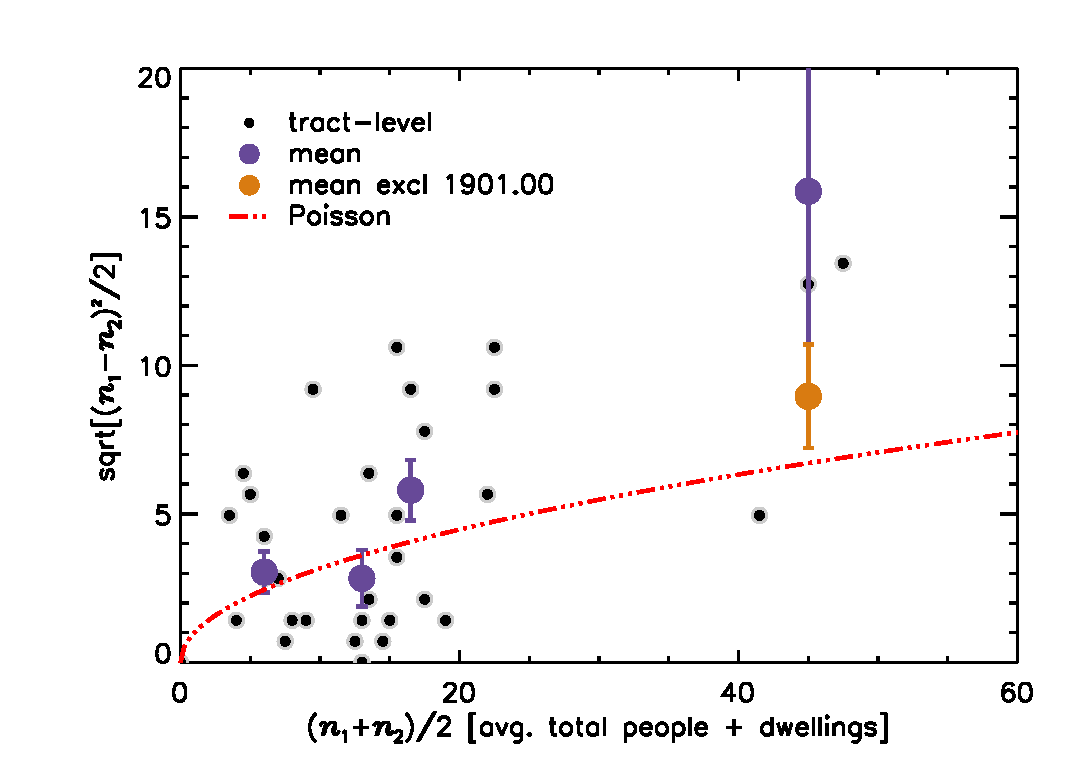
\includegraphics[width=\linewidth, trim = 1cm 0cm 0cm 0cm]{intDupeChar}\\
	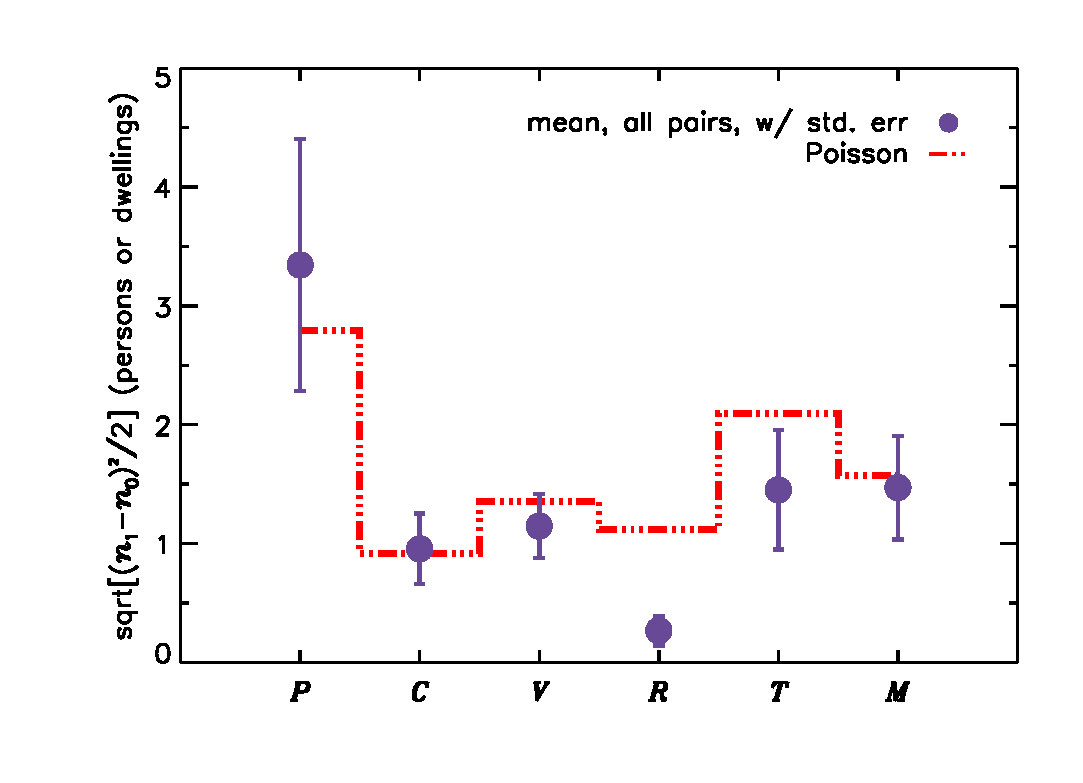
\includegraphics[width=\linewidth, trim = 1cm 0.5cm 0cm 0cm]{catDupeChar}
\caption{Intercounter result comparisons. {\it Top:} mean tract-level differences (large blue 
		points; 10-pair bins) are 1.4$\times$ the Poisson expectation (dot-dashes; 
		$\sqrt{\langle\nu\rangle}$); 1.3$\times$ excluding outlier tract 1901.00 (large green 
		point). Small points show pairwise differences. {\it Bottom:} mean category-level 
		dispersions are consistent with random errors except for RVs, which are identified 
		significantly more consistently. Only means are shown at bottom to reduce clutter.}
\label{fig:dupeChar}
\end{figure}

\subsubsection{Null Entries and Background Rates}
\label{sec:nulls}

Often, no persons or dwellings of a specific category are observed in a given tract. Probabilistically, 
these data are consistent with non-zero values for the true population. The Monte Carlo 
PDF reconstruction allows all such entries to fluctuate based on an assumed background rate,
$\sigma_{j}^{\rm bkg}$. 

Ideally, $\sigma_{j}^{\rm bkg}$ would derive from category variations in similar tracts defined 
by independent criteria. Sufficient data may exist to support that exercise, but it is beyond the scope 
of this analysis. Instead, we adopt a noise floor based on the counts expected if all members of a given 
category were distributed evenly across tracts:
\begin{equation}
	\sigma_{j}^{\rm bkg} \equiv \sqrt{\frac{1}{\ntracts}\sum_{\rm tracts}n_{j}}.
\end{equation}

While oversimplistic (Section \ref{sec:concentration}), this method works for any category
for which at least one individual/dwelling was observed in any tract. However, for categories for 
which this is not the case---unaccompanied minors and families, here---we set 
$\sigma_{j}^{\rm bkg}$ to the lowest non-zero value of the other categories (corresponding to 
TAY). The adopted backgrounds are thus: 
\begin{equation}
	\sigma_{j}^{\rm bkg}=\{3.1, 0.4, 0.4, 0.9, 1.3, 1.2, 2.8, 2.5, 0.4\}
\end{equation}
adults, TAY, unaccompanied minors, cars, vans, RVs, tents, makeshifts, and families per tract. 

Note that the above numbers are not added to null entries, but random draws from normal distributions
of that width. This treatment is somewhat arbitrary, but we employ it symmetrically---per-tract category 
inferences can be negative---so it does not bias the final estimate. Instead, it sets the upper limits of 
intrinsically rare categories and inflates aggregate uncertainties.

\begin{figure*}[t]
	\centering
	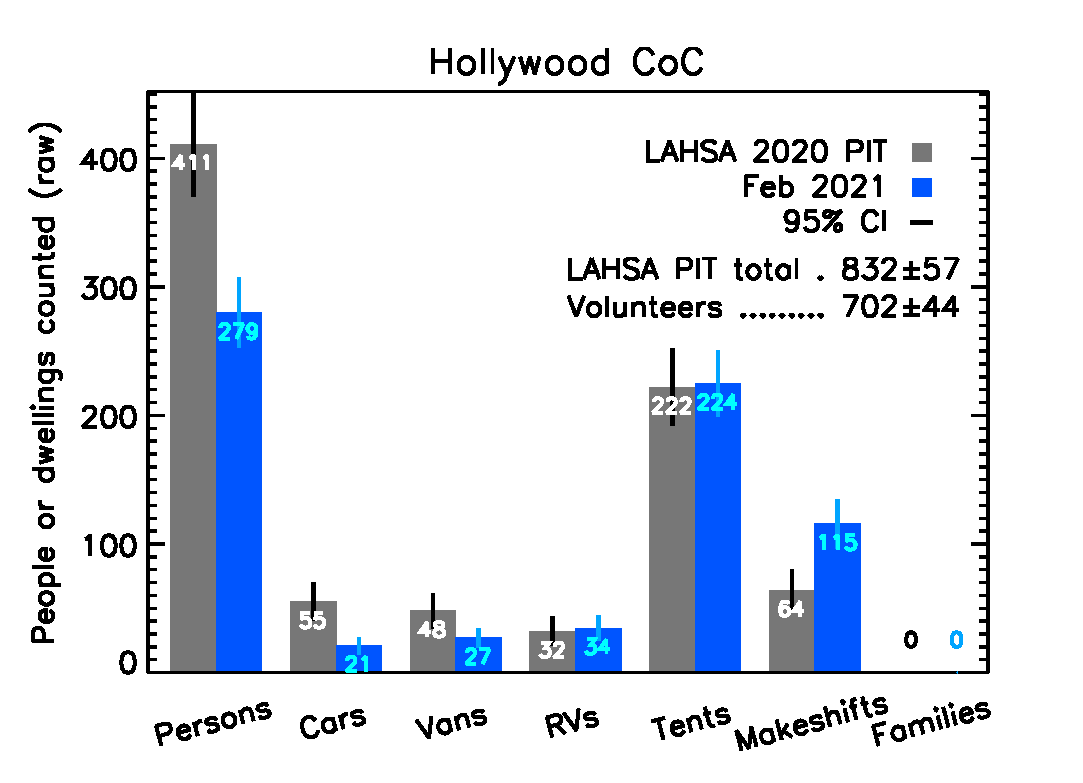
\includegraphics[width = 0.47\textwidth, trim = 1cm 0cm 0cm 0cm]{Hwood2021Bars}
	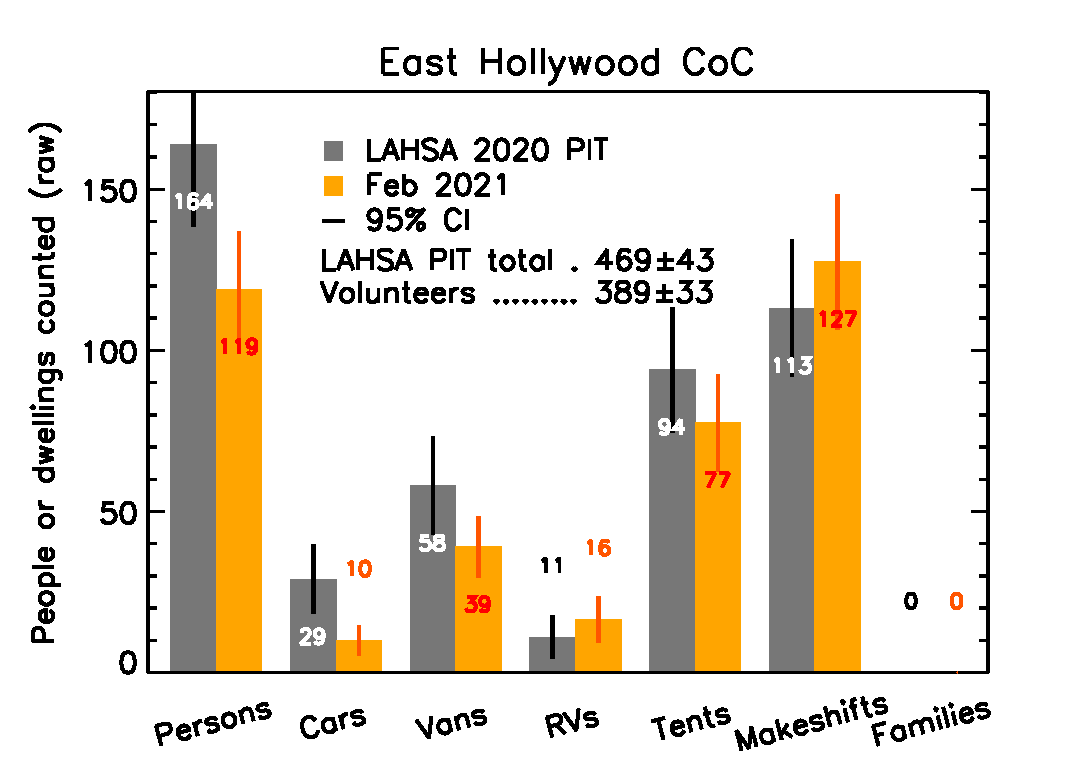
\includegraphics[width = 0.47\textwidth, trim = 0cm 0cm 1cm 0cm]{Eho2021Bars}
	\caption{Raw tallies of unsheltered persons and dwellings in Hollywood and East Hollywood
			(left/right) from the 2020 and 2021 PIT counts (grey/colors). Persons, cars, 
			and vans fell in both communities; RVs and tents stayed statistically flat. 
			Makeshift structures are the only category to show a potential common increase. 
			Overall, we identified 208 fewer people and dwellings compared to 2020,
			with similar 16\% decreases assessed by almost entirely independent teams
			in both communities. ``Persons'' are TAY+Adults.}
	\label{fig:rawCounts}
\end{figure*}

\begin{figure*}[t]
	\centering
	\includegraphics[width =0.47\linewidth, trim = 0.5cm 0cm 0cm 0cm]{hwoodHist}
	\includegraphics[width =0.47\linewidth, trim = 0cm 0cm 0.5cm 0cm]{ehoHist}
	\caption{2021 unsheltered population inferences compared to 2020 PIT results (red vertical lines) 
			using identical CVRTM weights (Table \ref{tbl:weights}).
			Orange dot-dashes show cumulative probabilities, suggesting a $\geq$95\%
			chance of a year-on-year decline.}
	\label{fig:communityPDFs}
\end{figure*}

\subsection{Duplicate Counts}
\label{sec:dupes}

Each volunteer tract in both communities (30) were assigned to at least two independent counting teams.
Four tracts additionally received a third pass. Pass 1 paired tracts by tract number. Pass 2 paired projected 
high-population tracts with ones geographically nearby. Pass 3 was the same as Pass 1 with 
pairings presented in reverse order, such that teams deployed simultaneously would likely start in different 
tracts. 

Results for one of the two teams assigned to tract 1925.20 could not be interpreted, making it the only
volunteer tract with one population estimate.

Figure \ref{fig:dupeChar} shows intercounter comparisons of raw counts (people+dwellings)
at the tract and category levels. Average offsets are close to Poisson expectations in all cases 
except for the highest occupancy tracts, where they are inflated by an outlier (see below).
Explicitly, $\langle\sqrt{(\nu_{1}-\nu_{2})^{2}/(\nu_{1} + \nu_{2})}\rangle=1.4$, where
$\nu$ is the total number of dwellings and people in a given tract returned by one of the teams. 
In the one instance where no persons or dwellings of any kind were identified (tract 1899.03), 
both teams agreed exactly.

The outlier is tract 1901.00, whose repeat measurements differ by $6.6\,\sigma$. There, 
one team counted $\{P,C,V,R,T,M\}=\{23,1,1,1,6,2\}$ while the other counted $\{77,15,10,1,6,6\}$. 
Abramson re-counted this tract on-foot 14 hours after the PIT tally, obtaining $\{36, 4, 6, 0, 8, 2\}$.
In total, this tally ($\nu_{\rm Abr}=56\pm7$) is within $1.9\,\sigma$ of the volunteers' mean 
($\langle\nu_{\rm PIT}\rangle=75\pm6$). As such, we retain the volunteer PIT estimate as-is. As illustrated in 
Figure \ref{fig:dupeChar}, top, the mean intercounter dispersion drops to $1.3\,\sigma$ if this tract is 
excluded.

In terms of categories, all dispersions are consistent with Poisson expectations except for RVs, where 
agreement is significantly better. Given their salience, this finding is reassuring if unsurprising.

%1901.00 inter-counter difference is 4.7 sigma (sqrt(delta) / root(n1 + n2) / root(2))

%\begin{itemize}
%%	\item All vol tracts counted at least twice;
%%	\item 4 tracts counted 3x;
%%	\item One recount DQed for quality flag (1925.20);
%%	\item Dupe statistics look pretty good. Mean abs discrepancy is consistent
%%		with zero given standard error on mean except for TAY (2.7 sigma) and RVs (3.8).
%%		Normalized differences ($|n_{1}-n_{2}|/\sqrt{n_{1}+n_{2}}$) are a little higher
%%		than $1\sigma$ ($CVRTM=[1.7, 1.1, -, 1.6, 1.4, 0.6, 1.2, 1.6, -]\sigma$), suggesting 
%%		a little more than poisson counting uncertainty, but LEA cross-checked the one
%%		highly discrepant ($\sim$8$\sigma$) tract, 1901.00, and found raw counts consistent
%%		with the average of the two nighttime datasets ($\sim$9:00 AM 26 Feb). 
%	\item Above holds true for 1912.01, which is in Hwood and also a SELAH recount tract. LEA
%		counted 51 totoal ppl/dwellings 12:30 P on 27 Feb vs 51 by vols night of count.
%\end{itemize}

No team counted tracts in both Hollywood and East Hollywood. As such, the volunteer counts
in those communities represent independent datasets. Including the professional-counted tracts, 
cross-talk comes from one tract in East Hollywood counted by a team that surveyed five 
tracts in Hollywood. We discuss intercommunity comparisons between volunteer and 
professionally counted tracts in Section \ref{sec:crossChecks}.

%{\bfr PRO TRACT RAW COUNT SHARE 2020: 44\% (23 tracts)
%
%PRO TRACT RAW COUNT SHARE 2021: 43\% (all tracts)}
%
%{\bfr Barely consistent if all of last year's vans and cars are still here. 95\% confidence limit $996\pm69$ can reach 1065 (v 1058) 
%in Hollywood, $598\pm 59= 657$ vs.\ 656 last yr in E.~Hollywood. BOTH AT 2020 SPA4 WEIGHTS!}


\section{Results}
\label{sec:results}

This section presents community- and aggregate-level estimates for the number of unsheltered people 
living in Hollywood and East Hollywood as of 25 February 2021. Sections \ref{sec:hWood} and \ref{sec:eHo} 
summarize our results, \ref{sec:comp} compares them to the 2020 LAHSA PIT estimates, 
\ref{sec:concentration} quantifies the population's geographic distribution, and \ref{sec:crossChecks}
presents cross-checks.

%Section \ref{sec:discussion} describes how 
%varying elements of Section \ref{sec:mc}'s analysis modulates these results.

\begin{table*}[t!]
\caption{Greater Hollywood 2021 PIT Unsheltered Data and Population Estimates}
\resizebox{\linewidth}{!}{%
\begin{tabular}{lcccccccccc}
\toprule
 & Adult & TAY & Car & Van & RV & Tent & Makeshift & {\bf 2021 Total} & {\bf 2020 Total} & {\bf Difference} \\ \cmidrule{1-11}
{\bf Hollywood} \\ %\cmidrule{1-1}
Counts & 280 & 2 & 21 & 28 & 38 & 230 & 116 & {\bf 715} & {\bf 831} & $\bf -14\%$ \\ %831
Inhabitants & 280 (28) & 2 (3) & 32 (11) & 51 (14) & 56 (14) & 339 (29) & 196 (24) & {\bf 956 (94)} & {\bf 1058} & $\bf -10\%\,(9\%)$\\% {\bf 1058}(76)
Category share & 29\% (3\%) & 0\% (0\%) & 3\% (1\%) & 5\% (1\%) & 6\% (1\%) & 35\% (3\%) & 20\% (3\%) & -- & -- & -- \\ \cmidrule{1-11}
{\bf East Hollywood} \\ %\cmidrule{1-1}
Counts & 114 & 4 & 10 & 39 & 16 & 77 & 127 & {\bf 389} & {\bf 469} & $\bf -17\%$ \\
Inhabitants & 114 (19) & 4 (4) & 15 (8) & 70 (15) & 24 (9) & 115 (19) & 216 (23) & {\bf 557 (83)} & {\bf 656} & $\bf -15\%\,(12\%)$\\% (60)
Category share & 20\% (3\%) & 1\% (1\%) & 3\% (1\%) & 13\% (3\%) & 4\% (2\%) & 20\% (3\%) & 39\% (4\%) & -- & -- &--
\\ \bottomrule
\end{tabular}
}
\caption*{Parentheses denote 90\% uncertainties 
(binomial for categories). Uncertainties larger than estimates imply only upper limits are available. Marginalized
upper limits imply $<$3 unaccompanied minors and families in either community.}%$^{\rm a}$ Excludes tract 1919.02, which was not counted. 
\label{tbl:summary}
\end{table*}

\subsection{Hollywood}
\label{sec:hWood}

Counters identified $\nch\pm45$ (95\% CI) persons and dwellings in the 22 census tracts 
comprising the Hollywood Community. Modulated by the baseline CVRTM weights, these 
estimates imply a total unsheltered population of $\nh$ people 
(90\% CI; Figure \ref{fig:communityPDFs}, left), with the plurality (35\%) living in tents 
(Table \ref{tbl:summary}; Figure \ref{fig:rawCounts}, left). The five tracts counted by professional 
teams---largely along the US 101 corridor---comprised 41\% of raw counts and 42\% of inferred 
unsheltered people. Tract 1910.00 (pro-counted) had the most people and dwellings (123; 170
total population); 1899.03 had the fewest (0; $<$12 total population). %These tracts also bracket the population statistics. 


\begin{figure*}[]
	\centering
	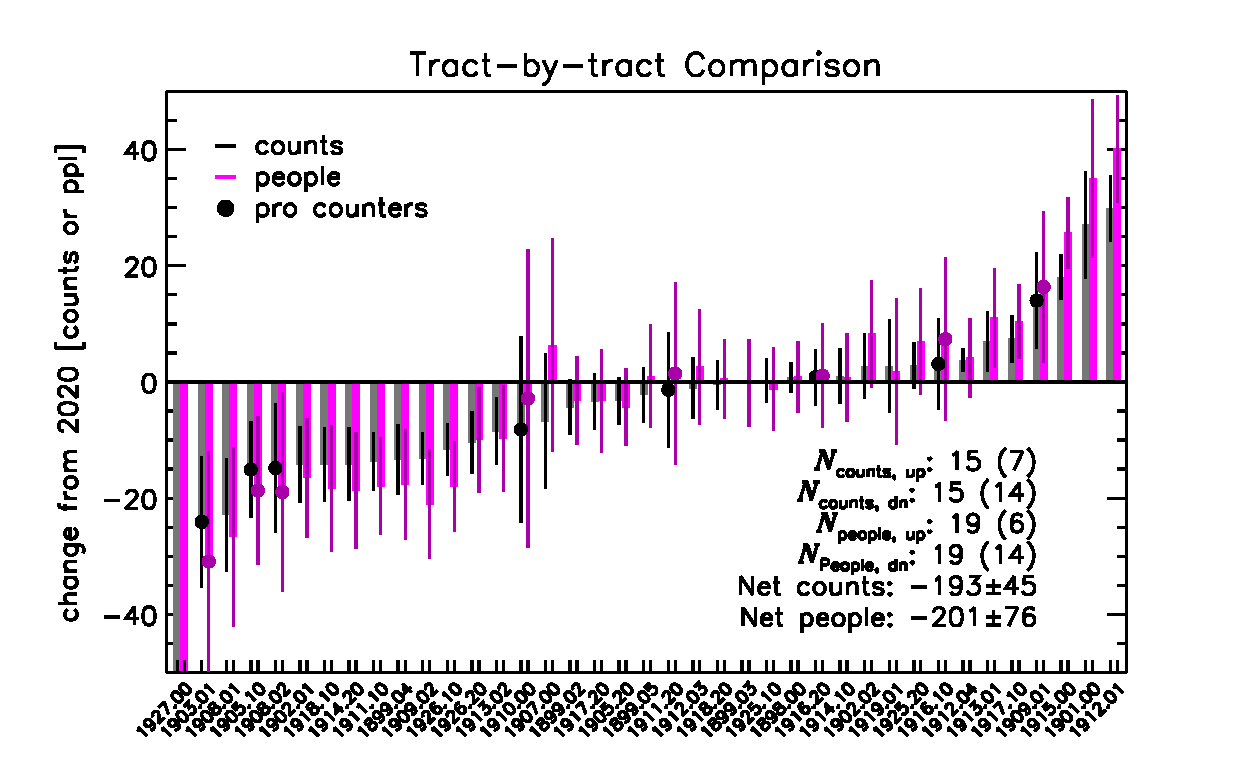
\includegraphics[width = 0.9\linewidth, trim = 0cm 0cm 0cm 0cm]{tractsYrYr}
	\caption{Compared to 2020, the 2021 PIT \Count\ identified 7 tracts with significantly more
			persons/dwellings, 14 with fewer (purple). The same holds for total unsheltered 
			population (orange; parentheses denote 1\,$\sigma$-significant changes). 
			Circles denote professional-counted tracts (1 increase; 3 declines). Net, 
			we identified about 200 fewer persons+structures or unsheltered 
			people. Tract 1927.00 saw the biggest decline (over 120 people; Section \ref{sec:discussion}), and
			may drive all of East Hollywood's inferred change from 2020.}
	\label{fig:tractYrYr}
\end{figure*}
%summing the tract level data returns the official community summary stats to within \pm 1 unit
% in all categories except vans, which are high in E. Ho by 4 counts -> 7 ppl; see int2020.pro

Modifying the CVRTM weights from the baseline SPA4/CD13 values to their 
\href{https://www.lahsa.org/documents?id=4693-2020-greater-los-angeles-homeless-count-cvrtm-conversion-factors}
{SPA4-wide} values lowers Hollywood's inferred total unsheltered population to $933\pm68$ people; applying
an updated tent weight based on a survey in Hollywood raises it to $964\pm118$ people (Section
\ref{sec:comp}). Neither shift is significant.

\subsection{East Hollywood}
\label{sec:eHo}

Counters identified $\nce\pm33$ (95\% CI) persons and dwellings in the 18 census tracts 
comprising East Hollywood. Modulated by the baseline CVRTM weights, these estimates imply 
a total unsheltered population of $\ne$ people (Figure \ref{fig:communityPDFs},
right), with the plurality (39\%) living in makeshift structures (Table \ref{tbl:summary}, 
Figure \ref{fig:rawCounts}, right). The four tracts counted by professional teams comprised 46\% of 
those counts and 47\% of inferred unsheltered people. Tract 1927.00 (pro-counted) had the 
most people and dwellings (87; 129 total population); 1912.04 had the fewest 
(5; $<$16 total population). 
%These tracts also bracket the total population statistics. 
%The plurality of counts were of makeshift structures---statistically 
%consistent with the number of persons identified on the street---followed by tents 
%(Figure \ref{fig:rawCounts}, right).

Modifying the CVRTM weights from the baseline SPA4/CD13 values to the SPA4-wide values 
lowers East Hollywood's inferred total unsheltered population to $539\pm59$ people; applying
the updated tent weight raises it to $559\pm87$ people. Neither shift is significant.

%\begin{figure*}[]
%	\centering
%	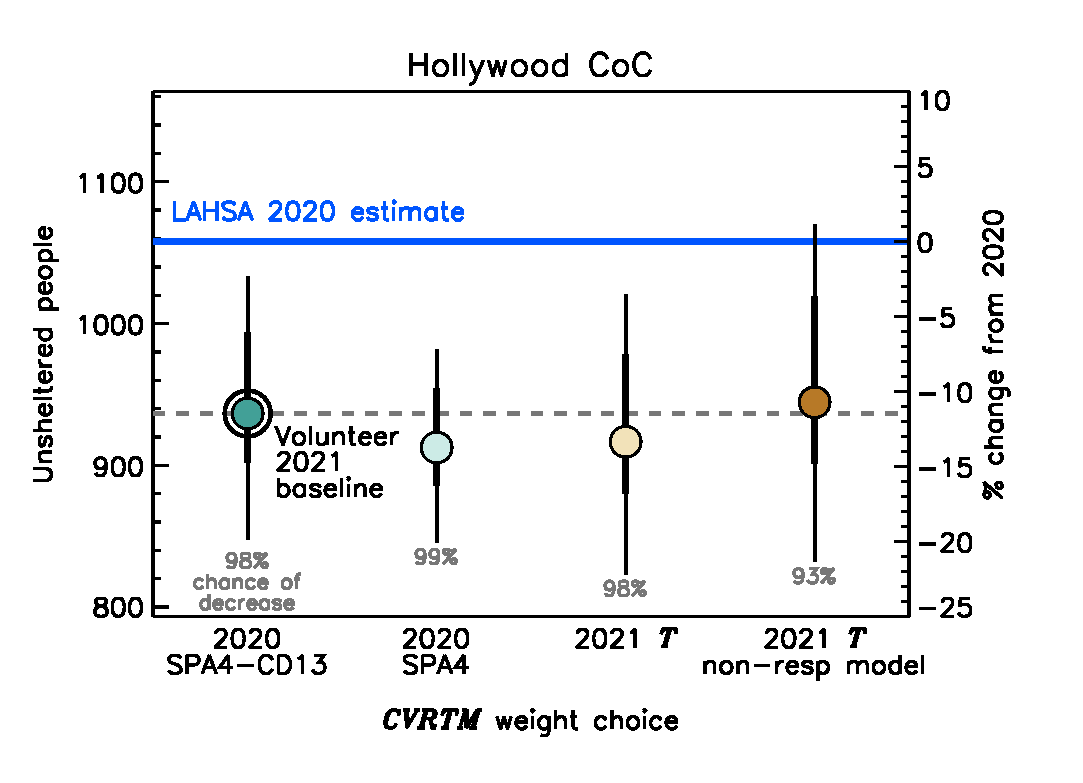
\includegraphics[width = 0.48\textwidth, trim = 0cm 0.5cm 0cm 0cm]{hwoodFinal}
%	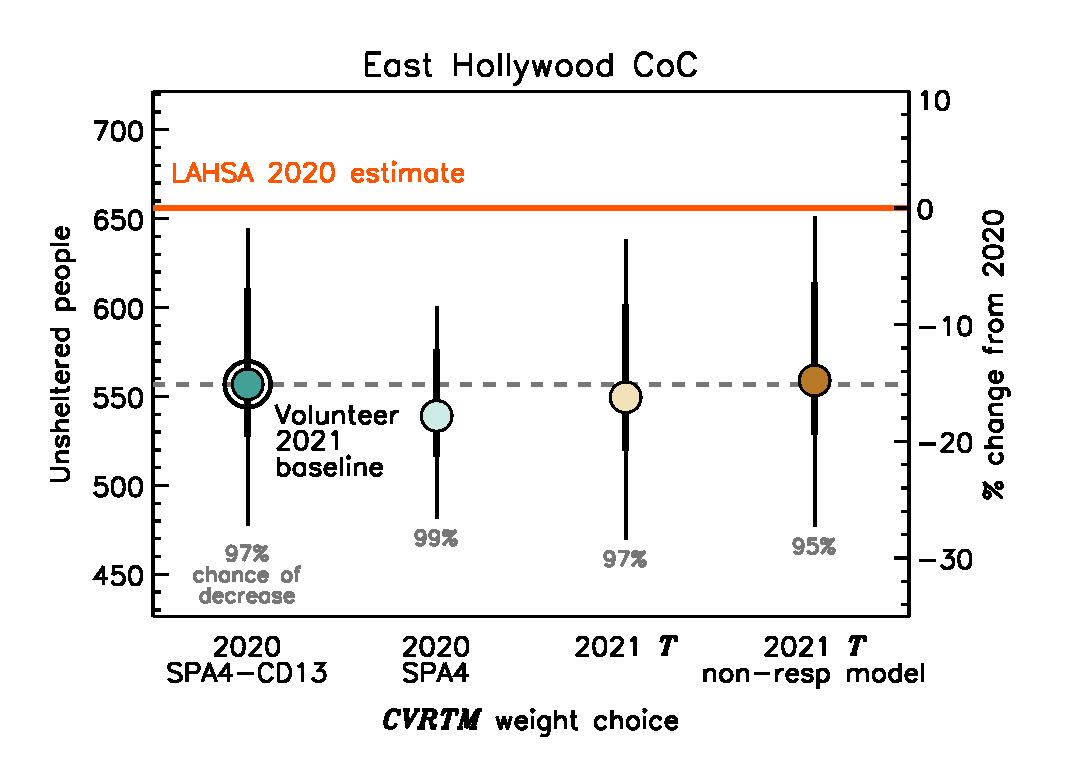
\includegraphics[width = 0.48\textwidth, trim = 0cm 0.5cm 0cm 0cm]{ehoFinal}	
%	\caption{Unsheltered populations in Hollywood (left) and East Hollywood (right) 
%			as functions of CVRTM weights. The baseline estimate uses the same weights as the 
%			2020 LAHSA Community Summaries. Using SPA4 weights or replacing the tent 
%			weight, $T$, with results from a survey conducted in Hollywood yields consistent
%			results. All imply at least a 93\% chance that unsheltered homelessness has fallen
%			by some amount, with likely declines of $12\%\pm9\%$ and $15\%\pm12\%$
%			in Hollywood and East Hollywood, \resp.}
%	\label{fig:wtComp}
%\end{figure*}


%\begin{figure}[]
%	\centering
%	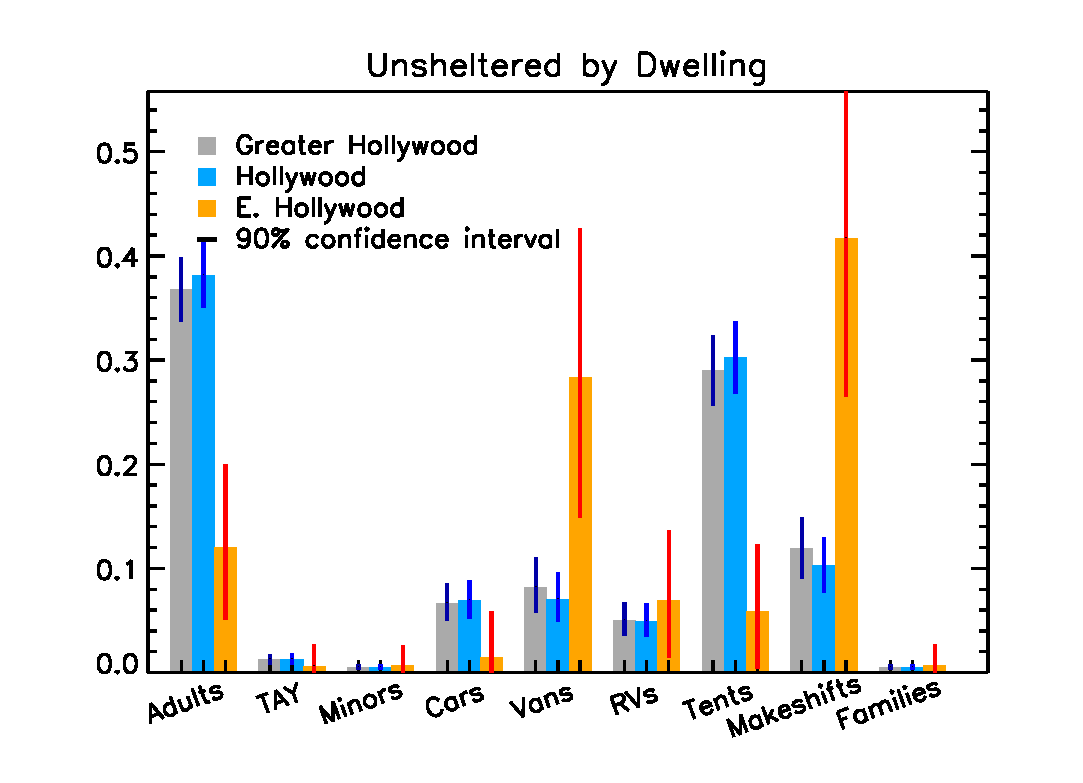
\includegraphics[width =\linewidth]{allTracts/allBreakdownBar}
%	\caption{}
%	\label{fig:popFracs}
%\end{figure}

\subsection{Comparison to 2020}
\label{sec:comp}

The official LAHSA estimates from the 2020 PIT count are overplotted in Figure \ref{fig:communityPDFs} 
as red vertical lines in each panel: 1058 unsheltered people in Hollywood, 656 in East Hollywood.
Our baseline inferences suggest a $>$95\% probability that the current population has fallen from 
those levels. Using the PDFs' medians and 90\% CIs, we infer declines of $\dh$ and 
$\de$, \resp. 

Figure \ref{fig:tractYrYr} shows the tract-level changes in counts and inferred populations as
geographically illustrated in Figure \ref{fig:map}. We find significant gains in 7 tracts and significant 
declines in 14, resulting in net changes of $-199\pm45$ and $-218\pm71$ counts or people, \resp.\footnote{Tract-level 
CVRTM counts inferred from \href{https://www.lahsa.org/data?id=45-2020-homeless-count-by-community-city}
{LAHSA's data portal}. We verified that they sum to the correct community totals.} 
Tract 1912.01 saw the largest year-on-year gain (Barnsdall Park; $+40$ people), tract 
1927.00 the largest loss (US 101; $-125$ people). Both are located in East Hollywood.

Tract 1927.00 is unique (Section \ref{sec:discussion}). Foremost among the reasons why is that its precipitous 
decline since 2020 can account for all of East Hollywood's total unsheltered population change. It is also the only 
tract assessed by a team that worked in both communities. If it is excluded, we infer $427\pm61$ unsheltered 
people in E.~Hollywood vs.\ 407 in 2020. Person/dwelling trends remain similar to those in 
Hollywood regardless of whether 1927.00 is examined, however (Figure \ref{fig:proVolComp}).
%368.808      426.952      491.580
%We speculate as to why these 
%tracts, specifically, saw such changes in Section \ref{sec:discussion}, along with why counts of rough
%saw particularly large declines.

Given the deficit in raw counts, it seems unlikely that reasonable modifications to the CVRTM weights 
will qualitatively affect our inferences. Nevertheless, due to the high proportion of people living in tents and 
makeshift structures, $w_{T}$ and $w_{M}$ are the largest potential error sources. 

To constrain their evolution
from last year, \href{https://selahnhc.org}{SELAH} outreach teams surveyed 47 tents (38 responses) 
in Hollywood on 28 Feb. This exercise yielded a mean occupancy of $w_{T}=1.39\pm0.14$ people per tent, 
or $w_{T}=1.50\pm0.22$ if non-responses are assumed to have anywhere from 0 to 4 occupants, each. 
While neither the full 2021 PIT area nor $w_{M}$ has been assessed,
%\footnote{$w_{M}=1.75\pm0.66$ was estimated using four makeshifts on 14 March but the sample size precludes.} 
the above values are consistent with the 2020 estimate of $w_{T}=1.48\pm0.11$. Neither adopting the 
updated $w_{T}$ value nor replacing all weights with the last SPA4-wide values leads to less than a
89\% chance of a decline in unsheltered populations compared to 2020. %93\%

%Figure \ref{fig:wtComp} illustrates the impact of various CVRTM choices, including the above. All cases imply at 
%least a 93\% chance of decline compared to 2020.

We encourage robust efforts to update the CVRTM weights, but the changes required to null the decline we find
are substantial. Only $w_{T}$ and $w_{M}$ can reasonably achieve it. These must rise to 2.1 and 
2.5 people from 1.5 and 1.7 people, \resp, in 2020. Not withstanding the above survey, such $\sim$45\% increases 
in {\it mean} occupancies seem unlikely. While 2021 is unprecedented in many ways, no SPA4/CD13 
CVRTM weight has changed by more than $\sim$30\% year-on-year since 2018.\footnote{$w_{R}$ fell from 
$\sim$2 to $\sim$1.4 between 2019 and 2020.}
% especially as known COVID-related tent distribution efforts have pushed 
%in the opposite direction (Section \ref{sec:discussion}). 

Largely, our results reflect the fact that persons seen on the street fell by $\sim$30\% (Figure 
\ref{fig:rawCounts}). Cars and vans are also down from last year by more than the number of 
safe parking spaces (Section \ref{sec:crossChecks}). Only makeshift structures show a potential 
common gain. All told, however, the total number of dwellings remained roughly flat. Although 
uncertainties in East Hollywood and effects from tract 1927.00 are large, Figure \ref{fig:proVolComp} 
reveals this trend to be common across communities and areas counted by volunteers or professionals. 
Such consistencies in nearly independent datasets suggest the results are robust. 
%Section \ref{sec:crossChecks} presents further checks.

%(Unsheltered people make up 3.5\% of tract 1907.00's total population, according to 2020 estimates
%from the US Census.)
%combined with COVID-related relaxations of tent-folding ordinances and the de-scoping of
%sanitation efforts suggests that the 

\subsection{Geographic Concentration}
\label{sec:concentration}

Everyday experience (and Figure \ref{fig:map}) confirms that unsheltered homelessness is
unevenly distributed. This statement is worth quantifying so that arguments over, e.g., the 
placement of new housing facilities may be grounded in data. Figure \ref{fig:gini} is one attempt to 
do so. 

Combining our PIT \Count\ with 2020 \href{https://geomap.ffiec.gov/FFIECGeocMap/GeocodeMap1.aspx}
{US Census} data, we compare the distribution of unsheltered Angelenos vs.\ all Angelenos in Greater
Hollywood. The top panel shows the proportion of people in a given tract that are unsheltered. This fraction 
spans 0\% to over 4\%, with a mean near 1\%---1.4$\times$ higher than 
\href{https://www.lahsa.org/documents?id=4680-2020-greater-los-angeles-homeless-count-city-of-los-angeles}
{LA's global unsheltered fraction} in Jan.~2020 (assuming 4M Angelenos).

The bottom panel shows the cumulative contribution of each tract to Greater Hollywood's
total and unsheltered populations. If people were equitably distributed, the curves would 
form a diagonal line of unit slope, yielding a Gini coefficient $c_{\rm Gini}=0$. 
The total population in Greater Hollywood has $c_{\rm Gini}\simeq0.1$---50\% of people 
living 40\% of tracts---close to evenly distributed. The unsheltered population, 
on the other hand, has $c_{\rm Gini}=0.44\pm0.02$---50\% of people living in 20\% of 
tracts---analogous to those describing income inequality in 
\href{https://en.wikipedia.org/wiki/List_of_countries_by_income_equality#UN,_World_Bank_and_CIA_list_\%E2\%80\%93_income_ratios_and_Gini_indices}{Rwanda, Philippines, or Malawi}. Such a concentration 
of lived trauma, real poverty, and the attendant externalities of unsheltered homelessness 
should condition equity-driven policymaking.

\begin{figure}[t]
	\centering
	\includegraphics[width =\linewidth, trim=0.75cm 0.25cm 0cm 0cm]{volProfComp}
	\caption{Year-on-year trends in pro- and vol-counted tracts are consistent in both 
			communities, though uncertainties in East Hollywood are large and
			effects from tract 1927.00 are strong. While dwellings stayed roughly flat, 
			persons were down significantly. The volunteer (purple) and pro results 
			with tract 1927.00 removed (turquoise, dashed at right) represent
			completely independent datasets. Errors are $1\,\sigma$.}
	\label{fig:proVolComp}
\end{figure}

\begin{figure}[t!]
	\centering
	\includegraphics[width =\linewidth, trim = 0cm 0cm 0cm 0cm]{totPopFrac}\\
	\includegraphics[width =\linewidth, trim = 0cm 0.5cm 3.5cm 0.25cm]{gini}
	\caption{{\it Top:} 0\% to over 4\% of each tract's total population is experiencing unsheltered
			homelessness in Greater Hollywood. The mean of $\sim$1\% is about 1.4$\times$ above
			the citywide average. {\it Bottom:} unsheltered homelessness is much more concentrated 
			than the general population, with 50\% of unsheltered persons+dwellings confined to 
			$\sim$20\% of census tracts (vs.\ 40\%	for all residents). The implied Gini coefficient
			is about that describing income inequality in 
			\href{https://en.wikipedia.org/wiki/List_of_countries_by_income_equality}
			{The Philippines}.}
	\label{fig:gini}
\end{figure}

\subsection{Cross-checks}
\label{sec:crossChecks}

Multiple cross-checks involving independent counters and external datasets suggest 
that the raw counts from our 2021 PIT \Count\ are accurate. The validating data are also
available at {\bfr website}.

\subsubsection{Internal checks}

Figure \ref{fig:dupeChar}'s comparisons of the count's 37 duplicate tract measurements suggest 
per-tract and -category counting uncertainties are consistent with the random errors built into the analysis. 
There is thus no strong evidence that counters were biased in identifying unsheltered persons or dwellings. 
Of course, the data do not preclude systematic errors in identifying, e.g., cars and 
vans---which can be difficult at night---but Figure \ref{fig:proVolComp} illustrates that, at least across all
dwellings, volunteers and professionals saw consistent trends. As the professional tracts were surveyed 
on foot and in daylight, such consistency suggests that biases are not large. Post-facto independent 
measurements of key geographies suggest this, too.

\subsubsection{External checks}

Three census tracts were re-surveyed in detail, none of which yield evidence of a PIT undercount:
\begin{itemize}
	\item 1901.00 -- {\it intercounter variability outlier}. Abramson
		  assessed this tract 14 hours after the PIT count (circa 9:00 AM) on foot with results 
		  $1.9\,\sigma$ lower than the volunteers' average (Section \ref{sec:dupes}):
		  $\{P,C,V,R,T,M\}_{\rm PIT} = \{50.0, 8.0, 5.5, 1.0, 6.0, 4.0\}$ vs.~
		$\{36, 4, 6, 0, 8, 2\}$.
	\item 1912.01 -- {\it largest increase}. Abramson assessed this tract on 
		27 Feb.\ circa 12:00 PM as part of SELAH monitoring. Results were consistent with 
		the PIT \Count\ to within $1\,\sigma$. $\{P,C,V,R,T,M\}_{\rm PIT}=\{18.5,0.5, 3.5, 1.5, 5.5, 12.0\}$ 
		vs.~$\{21,0,4,1,8,6\}$.
	\item 1927.00 -- {\it largest decrease}. Abramson assessed this tract
		on 4 March circa 8:30 AM by vehicle. Results were 35 inferred people lower than than the PIT 
		estimate, though with 9 additional vans sighted. Given this tract's configuration---intersecting 
		many freeway ramps and shoulders---the PIT survey was conducted on foot by outreach professionals. 
		As such, we take the recount only to suggest that the PIT data were likely not biased to induce an 
		artificial deficit of more than about $9\,w_{V}\simeq 16$ people.
\end{itemize}

Two larger-geography surveys concur:% quantitatively and qualitatively:
\begin{itemize}
	\item Biweekly data from \href{https://hollywoodpartnership.com/}{\it The Hollywood Partnership} 
		from 19 Feb.\ are consistent with PIT counts in a common tract (1902.02) and with an independent 
		recount of the entire Business Improvement District performed 28 Feb.\ by Abramson and 
		Kohan. These data also imply a decline from past values.
	\item Three additional tracts in Echo Park and Silver Lake monitored biweekly by SELAH since May 2020 
		show declines similar to that inferred for Greater Hollywood.
%		\footnote{Tract 1912.01 is also monitored by SELAH. Its
%		recount was conducted as part of that effort.} 
\end{itemize}
%
%A 27 Feb.\ recount of tract 1912.01 in East Hollywood conducted as as part of a
%		\href{https://selahnch.org}{SELAH} monitoring campaign agrees with our PIT value.% in unsheltered homelessness.
%

Finally, if the 49 safe parking spaces in or near the survey area\footnote{Per CD13 field deputy. 
 Includes Echo Park. Safe parking providers did not respond to an email query.} 
were occupied on 25 Feb., these locations probably went uncounted. Adding the implied 
$80\pm16$ total car and van dwellers to our results (equal mix) reduces the baseline chance of a 
decline in unsheltered people from 98\% to 89\%. %98\% to 92\%. 
%it  account for roughly half of the car+van deficit we see vs.~2020.

All of the above suggests that our results are reliable.
%Assumes equal mix of cars + vans.
%From Starkey: Hwood = 25, Eho = 10, EchoPk = 14; total = 49; total CD13 = 59 but I think it's reasonable
%to truncate at Echo Pk. It's 90% if you include all 59 spaces.

%		   P	C     V	    R	 T     M
%1901.00 -- 50    8    5.5   1     6      4 -- 2021, raw
%1901.00 -- 36    4     6     0     8      2 -- 26 Feb ABRAMSON 9.00 AM
%
%1927.00 -- 48    1      5     0    53    70 -- 2020, raw
%1927.00 -- 20    0     0     7     6     54 -- 2021, raw
%1927.00 -- 15     0     9     5    14    21 -- 4 Mar 2021 ABRAMSON 8.45 AM
%
%1912.01 --  18.5  0.5  3.5  1.5  5.5  12 -- 2021, raw
%1912.01 --  21     0      4     1     8      6  -- 27 Feb ABRAMSON 12.15 PM
%
%1902.02 -- 9      --     --     --     8   5.5 -- 2021, raw
%1902.02 -- 9      --     --     --    17    --  -- BID 2/19

% 1907.00 is also interesting in that total population stayed nearly the same but identified
% individuals and dwellings basically swapped: IND 73->38; CVRTM 31->70. This has a big impact
% on people's perceptions, and it's in a very high-traffic part of the community.

%The pro/vol trends are consistent everywhere except tract 1927.00, 
%			where pro counts dropped significantly more for both individuals and dwellings (esp.\ 
%			tents). 1927.00 comprises 22\% of total counts in East Hollywood. Unsheltered 
%			homelessness in that CoC was flat or rose slightly outside of that tract.}
%{\bfr 1927.00 is the tract with the PATH Madison PSH. Phase II opened in Jan 2020---leasing began May 
%2020---and is 120 units, some of which were filled from nearby folks but I dunno how many. LEA recounted 
%this tract 4 March at $\sim$9:00 AM and found 94 total population vs.\ pro's 129. Only place where
%LEA counted more objects was vans. Adding that to the pro total adds 16 people (9 vans).

%HOLLYWOOD -- Zero delta requires CVRTM mean occupancies of:\\
% - 5.00 ppl/car (from 1.51)
% - 5.00 ppl/van (from 1.77)
% - 4.00 ppl/RV (from 1.42)
% - 1.90 ppl/tent (from 1.48)
% - 2.53 ppl/mkshft (from 1.68)
%
%EAST HOLLYWOOD -- Zero delta requires CVRTM mean occupancies of:\\
% - 5.00 ppl/car (from 1.51)\\
% - 4.33 ppl/van (from 1.77)\\
% - 5.00 ppl/RV (from 1.42)\\
% - 2.78 ppl/tent (from 1.48)\\
% - 2.45 ppl/mkshft (from 1.68)

% ------ SUMMARY for HWOOD ------ 
%
%Total People (90%CI) .   936+/-92
%Fraction vs. last yr .   0.89+/-0.09
%Total counts..........   702
% > Adults    : 277 (39%), 277, (29%)
% > TAY       :   2 ( 0%),   2, ( 0%)
% > Minors    :   0 ( 0%),   0, ( 0%)
% > Cars      :  21 ( 2%),  31, ( 3%)
% > Vans      :  27 ( 3%),  47, ( 5%)
% > RVs       :  34 ( 4%),  49, ( 5%)
% > Tents     : 224 (31%), 330, (35%)
% > Makeshifts: 115 (16%), 193, (20%)
% > Families  :   0 ( 0%),   0, ( 0%)
%% Compiled module: MINMAX.
%Min/max ppl/tract ..... 0, 169
%Min/max counts/tract .. 0, 123
%
% ------ SUMMARY for EHO ------ 
%
%Total People (90%CI) .   556+/-83
%Fraction vs. last yr .   0.85+/-0.13
%Total counts..........   389
% > Adults    : 114 (29%), 114, (20%)
% > TAY       :   4 ( 1%),   4, ( 0%)
% > Minors    :   0 ( 0%),   0, ( 0%)
% > Cars      :  10 ( 2%),  14, ( 2%)
% > Vans      :  39 (10%),  68, (12%)
% > RVs       :  16 ( 4%),  23, ( 4%)
% > Tents     :  77 (19%), 114, (20%)
% > Makeshifts: 127 (32%), 214, (38%)
% > Families  :   0 ( 0%),   0, ( 0%)
%Min/max ppl/tract ..... 6, 129
%Min/max counts/tract .. 5, 87

\section{Discussion}
\label{sec:discussion}

\begin{figure}[t]
	\centering
	\includegraphics[width =\linewidth, trim = 1cm 0.5cm 0cm 0cm]{tract1907comp}
	\caption{An example of one of 11 tracts where tent+makeshift frequencies at least 
			doubled. 1907.00 lies in the heart of Central Hollywood, increasing the visual impact of this
			rise in dwellings, which was almost offset by a decline in identified persons
			on the street.}
	\label{fig:1907}
\end{figure}

As far as we can assess, the number of people experiencing unsheltered
homelessness in Greater Hollywood has fallen by roughly 10\% from its Jan.~2020 level. A number of factors 
may contribute to this decline, some COVID-related and some not.
%\footnote{917 and 491 people in Hollywood and E.~Hollywood, \resp.} 

\subsection{Government Initiatives}

Foremost among these are government programs aimed at moving people indoors and stanching inflow into 
homelessness. The two most salient are COVID-related: Project Roomkey and eviction moratoria.
%Note that Coordinate Entry System (CES) data will constrain all of the following scenarios.

\subsubsection{Eviction Moratoria}

We do not know how many people the moratoria have prevented from becoming homeless. However,
per the LAHSA Count report, nearly 83,000 people became unhoused in 2020 from LA County's pool 
of over 500,000 rent-burdened residents. Of these, $\sim$7500 could not be rehoused. Thus, if the eviction
moratoria reduced even 10\% of last year's inflow, extant mechanisms may have been able to place 
everyone who lost their housing under a new roof.

However, while our PIT data show a decline in unsheltered living, at $\sim$10\%, the implications for 
the period \href{https://www.latimes.com/california/story/2021-01-12/new-report-foresees-tens-of-thousands-losing-homes-by-2023}
{after the eviction moratoria lapse} are not necessarily rosy.

\subsubsection{Project Roomkey}

More information is accessible regarding Project Roomkey. Also according to the 2020 Count report, 
over 6000 unsheltered LA County residents became sheltered at some point between March and May of that year.
Examining only \href{https://www.lahsa.org/documents?id=4672-2020-homeless-count-council-district-13}
{CD13's} share of \href{https://www.lahsa.org/documents?id=4585-2020-greater-los-angeles-homeless-count-los-angeles-continuum-of-care-coc-}{LA County's unsheltered senior population} (6.5\%), perhaps 100 of Roomkey's 
\href{https://projectroomkeytracker.com/}{1608 occupied rooms} were filled with Greater Hollywood residents 
on the night of 25 Feb. If so, this would account for about half the inferred global reduction. 

Data from the Coordinated Entry System (CES) will constrain this scenario.

\subsubsection{A Bridge Home}

Unrelated to COVID, at least one \href{https://www.lamayor.org/ABridgeHome}{\it A Bridge Home} (ABH) 
opened between this year's and last year's PIT estimate whose catchment area spans nearly all of Greater 
Hollywood. Assuming 50\% capacity due to COVID precautions, the Riverside site can account for a further 
50 people exiting the unsheltered population.

However, COVID-related ``decompression'' of congregate living sites simultaneously reduced available beds in 
pre-existing shelters. Assuming 50\% reductions, we estimate that the five ABHs \href{https://arcg.is/0fy81}
{whose catchments touch Greater Hollywood}---Schrader, YWCA/Lodi (recently expanded), Gardner, Riverside, and 
Lafayette---constitute a net addition of just 33 beds (398 total, 116 gained, 83 lost to decompression). 

Local contributions can be larger, however. Tract 1927.00---which saw the largest year-on-year 
decline---overlaps with three ABH catchments, two of them new. As many as 89 beds may thus have become
available to that tract's unsheltered residents, corresponding to $\sim$70\% of that tract's inferred population change.
% without considering any contributions from a new PATH permanent supportive housing site (see below).

CES data will constrain this scenario.

\subsubsection{Permanent Supportive Housing}

Finally, the leasing of 120 new PATH permanent supportive housing units may also have contributed. 
That site happens also to be located in tract 1927.00. We do not know how many of its rooms went to Greater Hollywood 
residents or those of its home tract, but any that did would help drive the declines we infer in both.

CES data will constrain this scenario.

\subsection{Other Losses}

\subsubsection{Geographic Leakage/Edge Effects}

Our PIT \Count\ covered a limited geography. As such, people exiting Greater Hollywood to nearby communities
is an obvious potential loss having nothing to do with housing initiatives. In border tracts, this means nothing more than
crossing the street. 

Tract 1927.00 is, again, special in this regard as two of its edges are borders, and there is additionally a substantial 
community of unsheltered Angelenos opposite its eastern flank. We cannot exclude the possibility that (its) residents simply 
left, but upcoming grassroots PIT counts in Mid City and Silver Lake---which bound Greater Hollywood to the southwest and 
east, \resp---may provide insights.

\subsubsection{Deaths}

An unfortunate but inevitable source of population loss is death. While COVID mortality rates are
\href{https://www.medrxiv.org/content/10.1101/2021.03.05.21253019v1}{far higher} among people
experiencing homelessness relative to the general population, \href{http://publichealth.lacounty.gov/media/coronavirus/docs/SummaryReport_People_Experiencing_Homelessness.pdf}
{Dept.\ of Public Health statistics} suggest that $\sim$200 unhoused LA County residents had succumbed to the 
disease by the time of the PIT count, subordinating its impact to other causes.

Instead, \href{http://publichealth.lacounty.gov/chie/reports/HomelessMortality2020_CHIEBrief_Final.pdf}{drug overdoses},
particularly from methamphetamine, likely dominate. Based on data spanning only the first seven months of 2020, overdoses had
killed 929 people experiencing homelessness---a rate 7.6$\times$ higher than COVID to that point.

All told, deaths of people experiencing homelessness increased by 26\% from Jan.\ through July 2020 compared to 
the same interval in 2019. A more rigorous analysis is needed to determine the extent to which those deaths contributed 
qualitatively to the decline we infer, but, quantitatively, they must have.

\subsection{Objective Support for Subjective Trends}

The authors of this report did not anticipate a decline in Greater Hollywood's unsheltered population.
The feeling accumulated over the course of 2020 was one of a meaningful, if not dramatic worsening in the
state of homelessness. The PIT data provide hints as to how these subjective and objective conclusions may be
reconciled.

Principally, smaller scales tell different stories than the community level results. Eleven tracts---28\%---saw at 
least a doubling in their number of tents and makeshift structures, with a mean increase of $\sim$10 such dwellings
per tract.\footnote{Tracts 1899.04, 1902.02, 1907.00, 1911.20, 1912.01, 1913.01, 1913.02, 1914.10, 1915.00,
1916.10, 1917.20.} As such, the {\it visual salience} of unsheltered living increased markedly in many places. Moreover,
this quantitative growth was qualitatively amplified by LAPD's \href{https://clkrep.lacity.org/onlinedocs/2020/20-0147_misc_3-17-20_p.pdf}{suspension of LAMC 56.11} enforcement during COVID. 
Ordinarily, this law requires tents to be collapsed during the day. Without it, the impression of homelessness might 
increase even in areas where the number of tents {\it declined} as those that remained would be newly salient.
The effect in places where tents doubled is obvious. Tracts 1907.00 and 1912.01 are two such places.
%Six tracts saw at least a 
%50\% increase in the number of dwellings. Of these, four saw more than 100\% gains.\footnote{Tracts 1902.02, 
%1907.00, 1912.01, 1915.00, accounting for nearly 9\% of all street dwellings and 16\% of all counts.} % 1925.20

Tract 1907.00 is located in the heart of Central Hollywood's commercial district.\footnote{Fountain to Sunset to Franklin, 
Vine to Seward to Highland.}  Not only did dwellings double here, but it is one of four tracts wherein dwellings
and persons swapped shares of the unsheltered population compared to 2020. The swap was so precise in 1907.00
as to nearly conserve the total number of identified people+dwellings (Figure \ref{fig:1907}). This phenomenon would 
enhance the impression of unsheltered living even as the population as a whole remained unchanged.

Meanwhile, tract 1912.01's population did not remain the same, but more than {\it tripled}, leading to the largest 
absolute gain vs.~2020. Containing Vermont Ave between Fountain and Hollywood Blvd, and Hollywood Blvd between 
Vermont and Normandie (Barnsdall Park), this tract, like 1907.00, is a high-traffic area, and so one of enhanced visibility. 

Even as overall numbers declined, the above local trends show how facts in key areas would support impressions
that the opposite occurred. This is to say nothing of deteriorations in the conditions of street living
for those unable to get indoors (see next section).

Finally, the above trends also provide some evidence of the impact of COVID-related tent distribution efforts 
by professional and volunteer service providers. Anecdotally, these are reported as robust despite the global 
number of tents remaining similar to 2020 levels. A concentration of tents in the above tracts combined with a 
substantial fraction going to replacing damaged or destroyed tents may have soaked up this source.

%Ancillary data from regularly monitored census tracts suggests that the date offset is unlikely to substantially 
%erode comparability between this and past datasets. Limited daytime recounts also suggest that 
%time-of-day effects are sub-dominant.

%1927.00 is actually in the catchment of 3 ABHs that were either new or expanded between PIT counts. 
%Lodi, however, did not fill its new beds, and Lafayette doesn't cover the whole tract, so we won't speculate.
%Nevertheless, technically, even at 50\% decompression, residents of 1927.00 may have been eligible 
%for any of 89 new ABH beds. It's also on the CoC boundary.

\subsection{Quality of Life Degradation}

If there are fewer people on the street today, their quality of life has doubtless degraded. 
COVID has restricted or eliminated access to restaurant and park bathrooms, libraries (so 
\href{https://www.lapl.org/homeless-resources/the-source}{\it The Source} service days), Dept.~of Public Social Services 
(EBT, Medi-Cal), Dept.~of Motor Vehicles (ID replacement), and Dept.~of Mental Health facilities. Physical limitations 
on client access at hospitals has also hindered caseworkers from managing successful discharges. These 
harms are reflected by said 25\% increase in 
\href{https://www.latimes.com/california/story/2021-01-07/the-powerful-synthetic-opioid-fentanyl-is-behind-rising-deaths-in-the-homeless-population}{overdose deaths}, and amplified by the simultaneous 
\href{https://clkrep.lacity.org/onlinedocs/2020/20-0147_misc_3-17-20_p.pdf} {suspension or de-scoping} of city 
and state sanitation programs (which further increase the visual impact of aforementioned tent doublings). 

As such, while 2021 PIT data may support the efficacy of programs designed to reduce street 
homelessness, they do {\it not} suggest that the state of homelessness in Greater Hollywood has improved. 
In the fight to rebuild lives---as well as build homes---that fact must remain paramount.

\section{Summary}
\label{sec:summary}

Data from February 25, 2021 show that unsheltered homelessness has fallen in Hollywood and 
East Hollywood  by $10\%\pm9\%$ and $15\%\pm12\%$, \resp, compared to the 2020 LAHSA PIT 
Count (90\% CI). Multiple internal and external cross-checks support the quality of the 
data---30/40 tracts counted by multiple teams; consistency between volunteer- and 
professional-counted tract trends; consistency with external data---which
point to a 30\% drop in individuals seen on the street driving the year-on-year change.
The size of this shift makes it difficult for updates to dwelling occupancies to erase the 
community-scale declines we infer. 

We attribute the declines mainly to government initiatives---e.g., eviction moratoria, Project 
Roomkey---aimed at bringing or keeping people indoors. The opening of at least one {\it A Bridge Home} 
facility and new permanent supportive housing units likely also contributed. Data from the 
Coordinated Entry System will test these statements.

While community-level counts declined, 28\% of tracts saw at least a doubling in tents and 
makeshift structures. This phenomenon---amplified by suspension of LAMC 56.11 enforcement
and compounded by city and state sanitation de-scopings---may have contributed to qualitative 
perceptions that the state of homelessness worsened even as the numbers went down. Given 
COVID-related disruptions to health, hygiene, and social support services---these sentiments are also 
likely to be accurate. Especially in light of the lifting of eviction moratoria, much work remains to 
ensure everyone has a home in Hollywood.

\section*{}

LA acknowledges Dan Kelson for his analysis insights and all of the volunteers who participated
in the 2021 grassroots PIT \Count: Kate Adams;
Albert Andrade;
Rachel Andres;
Eleanor Atlee;
Thomas Atlee; 
Kate Aviv;
Elvina Beck; 
Clarissa Boyajian;
Peggi Carbonel;
Erin Casey;
Chip Clements;
William Clements;
Shreyansh Daftry;
Darius Derakshan;
Anthony Demarbiex;
Polly Estabrook;
Nicole Farley;
Mark Fishlowitz; 
Rana Ghadban;
Margaret Gillespie; 
Kali Ghazali;
Jane Gibson;
Charlotte Gordon;
Daniel Gracey;
Thomas Grogan;
Kate Hammond;
Lauren Hernandez;
Carter Hewgley;
Spencer Hillman;
Joan Howard;
Veronica Huerta;
Bill Kaplan;
Seth Kaplan;
Moira Kelly; 
Maryam Khoshreza;
Elizabeth Larson;
Kris Larson;
Jennifer Levin;
Marissa Levin;
Erica Levine;
Rhea K.~Mac;
Aditi Mahajan;
Thomas Mapp;
Erica Martin;
Kristian Melby;
Ren\'{e}e Mockhatel;
%Kerry Morrison;
Mackenzie Morrison;
Robert Morrison;
Chelsea Mottern;
Rebecca Nashleanas;
Andoni Nava;
Henry Perez;
Margarett Qaqish;
Kelly Reilly;
Elizabeth Roland;
Julia Roland;
Rich Sarian;
Allison Schallert; 
Jillian Schultz;
Robert Scott;
Priyanka Srivastava;
Carmen Stewart;
Devin Strecker; 
Ninoska Suarez;
Giuseppe Tantino;
Sierra Thomas; 
Leah Thompson; 
Dylan Tucker;
Ben Tysch; 
Matt Wait;
Brenna Wall;
Nadia Wehbe;
Delaney Wells;
Marilyn Wells.

\appendix

\section{Example Documents}

Figure \ref{fig:tractMap} shows an example tract map. 
Figure \ref{fig:tallySheet} shows the PIT tally sheet.
Figure \ref{fig:primer} shows the training summary provided to volunteer
teams on deployment.

\begin{figure}[t]
	\centering
	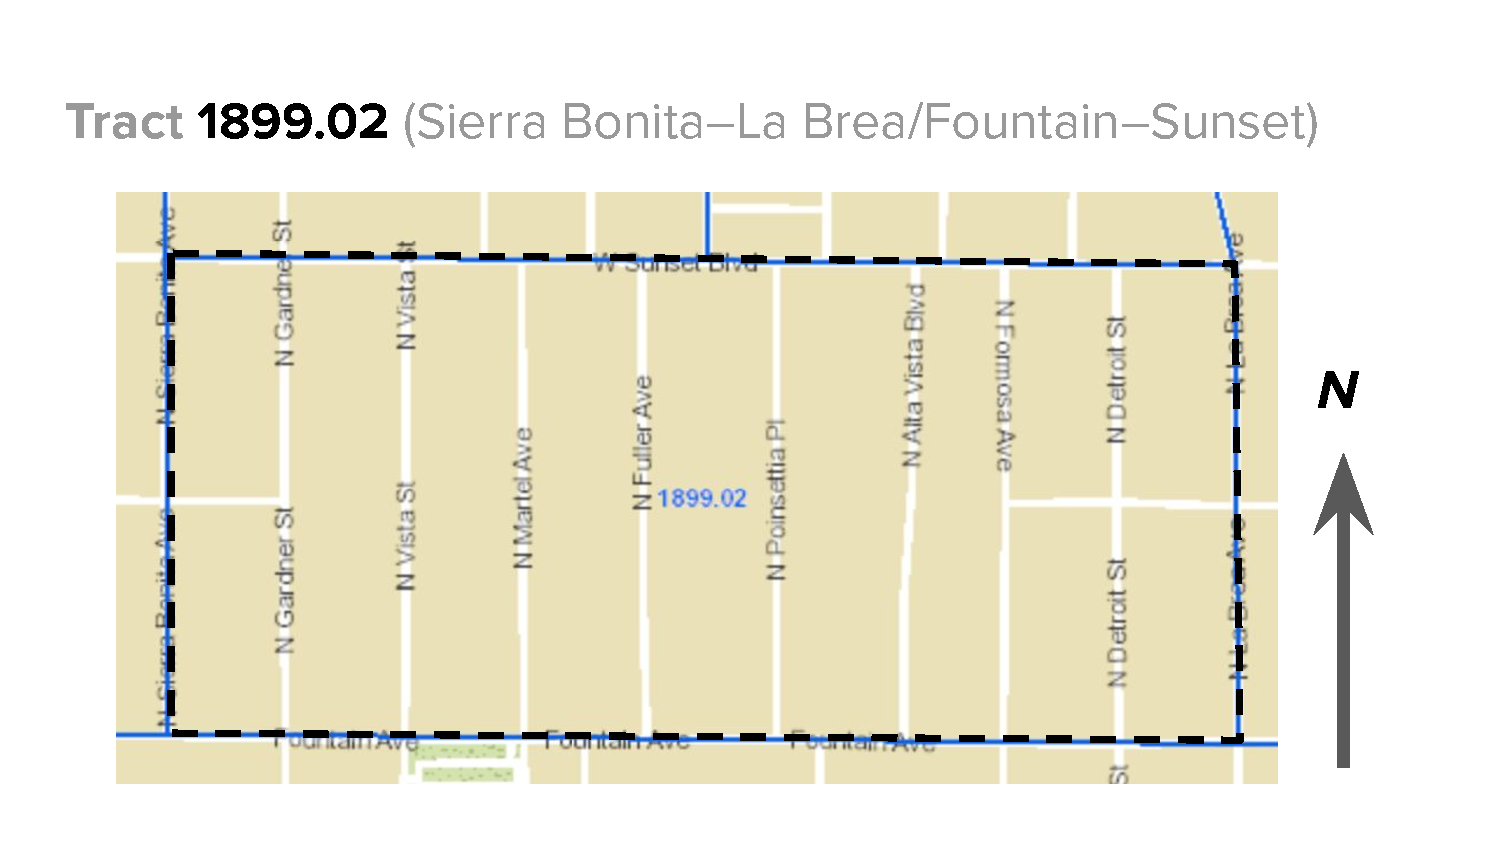
\includegraphics[width =\linewidth, trim = 1cm 0cm 1cm 0cm]{tractMap}
	\caption{Example Hollywood tract map.}
	\label{fig:tractMap}
\end{figure}

\begin{figure}[t]
	\centering
	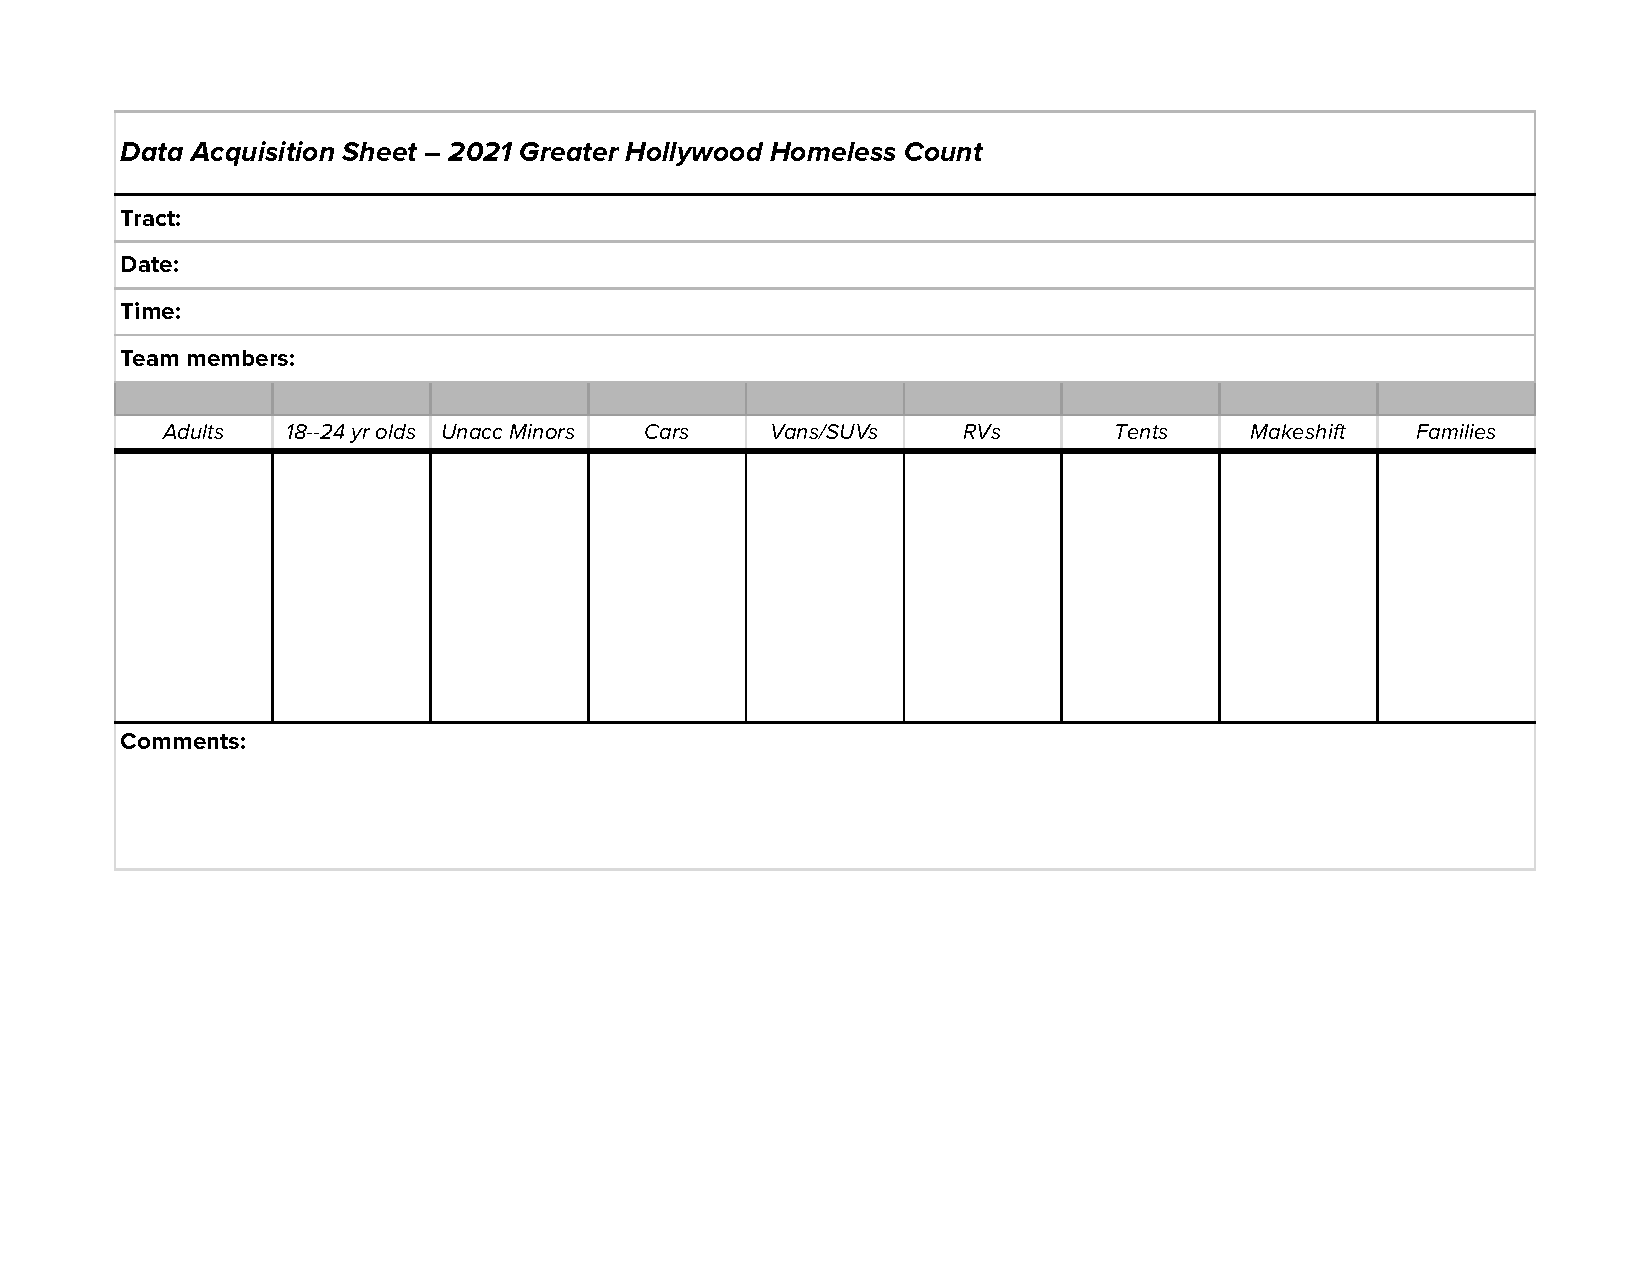
\includegraphics[width =\linewidth, trim = 2cm 6cm 2cm 0cm]{Hollywood2021CountDataSheet}
	\caption{Counter tally sheet/data collection tool.}
	\label{fig:tallySheet}
\end{figure}

\begin{figure}[t]
	\centering
	\includegraphics[width =0.85\linewidth]{primerFront}
	\caption{Count primer. The telephone number for the on-site emergency contact has been omitted for 
			privacy reasons.}
	\label{fig:primer}
\end{figure}

\section{Full Tract-level Results}

Tables \ref{tbl:allCount} and \ref{tbl:allPop} present counts and population inferences, \resp, for all 40 
Greater Hollywood census tracts. Professional surveying took place circa 3:00 PM on 25 Feb. Volunteers 
counted from 7 PM to 10 PM except in tract 1919.02, assessed the morning and evening of 16 March. 

\begin{table*}[t]
\caption{Census Tract-level Unsheltered Counts}
%\resizebox{\textwidth}{!}{%
\centering
\begin{tabular}{ccccccccccc}
\toprule
Tract & Community & Counter & Adults & TAY & Car & Van & RV & Tent & Makeshift & {\bf Total} \\ \cmidrule{1-11}
1898.00 & Hollywood & Vol &  3.3 &  0.3 &  0.0 &  0.7 &  0.0 &  1.3 &  0.0 &   5.7 \\
1899.02 & Hollywood & Vol &  4.3 &  0.0 &  0.0 &  1.3 &  2.7 &  4.0 &  1.3 &  13.7 \\
1899.03 & Hollywood & Vol &  0.0 &  0.0 &  0.0 &  0.0 &  0.0 &  0.0 &  0.0 &   0.0 \\
1899.04 & Hollywood & Vol &  9.5 &  0.0 &  0.0 &  1.0 &  0.0 &  2.5 &  2.0 &  15.0 \\
1899.05 & Hollywood & Vol &  3.0 &  0.0 &  3.0 &  4.5 &  1.0 &  2.0 &  0.0 &  13.5 \\
1901.00 & Hollywood & Vol & 49.5 &  0.5 &  8.0 &  5.5 &  1.0 &  6.0 &  4.0 &  74.5 \\
1902.01 & Hollywood & Vol & 14.5 &  0.0 &  0.5 &  0.0 &  0.0 &  2.5 &  1.5 &  19.0 \\
1902.02 & Hollywood & Vol &  9.0 &  0.0 &  0.0 &  0.0 &  0.0 &  8.0 &  5.5 &  22.5 \\
1903.01 & Hollywood & Pro & 10.0 &  0.0 &  0.0 &  0.0 &  0.0 & 19.0 & 22.0 &  51.0 \\
1905.10 & Hollywood & Pro & 13.0 &  0.0 &  0.0 &  0.0 &  4.0 &  6.0 &  4.0 &  27.0 \\
1905.20 & E.~Hollywood & Vol &  2.0 &  0.5 &  0.5 &  1.0 &  0.0 &  4.0 &  1.0 &   9.0 \\
1907.00 & Hollywood & Vol & 38.5 &  0.0 &  2.0 &  0.0 &  0.0 & 38.5 &  7.0 &  86.0 \\
1908.01 & Hollywood & Vol & 18.5 &  0.0 &  0.5 &  0.0 &  0.0 & 19.5 &  9.0 &  47.5 \\
1908.02 & Hollywood & Pro & 22.0 &  0.0 &  0.0 &  1.0 &  5.0 & 13.0 & 13.0 &  54.0 \\
1909.01 & Hollywood & Pro & 15.0 &  0.0 &  0.0 &  0.0 &  0.0 & 17.0 &  9.0 &  41.0 \\
1909.02 & Hollywood & Vol &  2.7 &  0.3 &  0.7 &  1.7 &  0.0 &  0.0 &  0.0 &   5.3 \\
1910.00 & Hollywood & Pro & 34.0 &  0.0 &  1.0 &  0.0 &  5.0 & 60.0 & 23.0 & 123.0 \\
1911.10 & E.~Hollywood & Vol &  4.0 &  0.5 &  0.0 &  0.0 &  0.0 &  2.5 &  0.5 &   7.5 \\
1911.20 & E.~Hollywood & Pro & 14.0 &  0.0 &  0.0 &  0.0 &  0.0 & 24.0 & 10.0 &  48.0 \\
1912.01 & E.~Hollywood & Vol & 17.5 &  1.0 &  0.5 &  3.5 &  1.5 &  5.5 & 12.0 &  41.5 \\
1912.03 & E.~Hollywood & Vol &  5.0 &  0.0 &  2.0 &  8.0 &  0.0 &  0.0 &  2.5 &  17.5 \\
1912.04 & E.~Hollywood & Vol &  3.0 &  0.5 &  0.5 &  1.0 &  0.0 &  0.0 &  0.0 &   5.0 \\
1913.01 & E.~Hollywood & Vol &  8.0 &  0.0 &  0.5 &  7.5 &  0.5 &  5.0 &  1.0 &  22.5 \\
1913.02 & E.~Hollywood & Vol &  5.5 &  0.0 &  0.5 &  0.5 &  0.5 &  3.5 &  6.0 &  16.5 \\
1914.10 & E.~Hollywood & Vol &  7.5 &  0.0 &  1.0 &  0.5 &  0.0 &  1.0 &  5.5 &  15.5 \\
1914.20 & E.~Hollywood & Vol &  4.0 &  0.0 &  2.0 &  4.5 &  1.0 &  3.0 &  2.0 &  16.5 \\
1915.00 & E.~Hollywood & Vol & 10.0 &  0.0 &  0.0 &  4.5 &  2.5 &  2.5 &  2.5 &  22.0 \\
1916.10 & E.~Hollywood & Pro &  6.0 &  0.0 &  0.0 &  1.0 &  1.0 &  2.0 & 22.0 &  32.0 \\
1916.20 & E.~Hollywood & Pro &  0.0 &  2.0 &  0.0 &  0.0 &  0.0 &  4.0 &  6.0 &  12.0 \\
1917.10 & Hollywood & Vol &  6.5 &  0.0 &  2.0 &  4.5 &  1.0 &  1.0 &  0.5 &  15.5 \\
1917.20 & Hollywood & Vol &  2.3 &  0.0 &  0.3 &  1.3 &  6.3 &  0.0 &  4.3 &  14.7 \\
1918.10 & Hollywood & Vol &  3.5 &  0.0 &  1.0 &  1.5 &  1.5 & 10.0 &  0.0 &  17.5 \\
1918.20 & Hollywood & Vol &  2.5 &  1.0 &  0.0 &  2.5 &  2.0 &  1.5 &  2.0 &  11.5 \\
1919.01 & Hollywood & Vol & 16.0 &  0.0 &  2.0 &  1.5 &  5.0 & 13.0 &  7.5 &  45.0 \\
1919.02$^{\ast}$ & Hollywood & Vol & 2.5$^{\ast}$ &  0.0$^{\ast}$ &  0.0$^{\ast}$ &  1.5$^{\ast}$ &  4.0$^{\ast}$ &  5.5$^{\ast}$ &  0.5$^{\ast}$ &  14.0$^{\ast}$ \\
1925.10 & E.~Hollywood & Vol &  4.0 &  0.0 &  1.5 &  1.0 &  1.5 &  0.0 &  1.5 &   9.5 \\
1925.20 & E.~Hollywood & Vol &  1.0 &  0.0 &  1.0 &  6.0 &  1.0 &  0.0 &  0.0 &   9.0 \\
1926.10 & E.~Hollywood & Vol &  2.0 &  0.0 &  0.0 &  0.0 &  0.0 &  3.5 &  0.5 &   6.0 \\
1926.20 & E.~Hollywood & Vol &  1.0 &  0.0 &  0.0 &  0.0 &  0.0 & 11.0 &  0.5 &  12.5 \\
1927.00 & E.~Hollywood & Pro & 20.0 &  0.0 &  0.0 &  0.0 &  7.0 &  6.0 & 54.0 &  87.0 \\
\bottomrule
\end{tabular}
%}
\caption*{$^{\ast}$Assessed 16 March. Raw counts from each tract coded as in Table \ref{tbl:tractStats}. 
		Fractions reflect averages over multiple counters.}
\label{tbl:allCount}
\end{table*}

\begin{table*}[t]
\caption{Census Tract-level Unsheltered Population Inferences}
\resizebox{\linewidth}{!}{
\begin{tabular}{ccccccccccc}
\toprule
Tract & Community & Counter & Adults & TAY & Car & Van & RV & Tent & Makeshift & {\bf Total}\\ \cmidrule{1-11}
1898.00 & Hollywood & Vol &  3.3 (1.7) &  0.0 (0.6) &  0.0 (2.2) &  0.0 (1.5) &  0.0 (2.8) &  1.9 (1.6) &  0.0 (7.0) &   6.9 (8.4) \\
1899.02 & Hollywood & Vol &  4.3 (2.0) &  0.0 (0.7) &  0.0 (2.3) &  2.3 (2.2) &  3.8 (2.5) &  5.9 (2.9) &  2.2 (2.0) &  18.7 (5.8) \\
1899.03 & Hollywood & Vol &  0.0 (5.2) &  0.0 (0.7) &  0.0 (2.2) &  0.0 (3.9) &  0.0 (2.8) &  0.0 (6.8) &  0.0 (7.1) &   0.0 (12.3) \\
1899.04 & Hollywood & Vol &  9.5 (3.6) &  0.0 (0.7) &  0.0 (2.3) &  0.0 (2.2) &  0.0 (2.7) &  3.7 (2.7) &  3.3 (3.0) &  18.3 (7.0) \\
1899.05 & Hollywood & Vol &  3.0 (2.0) &  0.0 (0.7) &  4.4 (3.3) &  7.7 (5.4) &  0.0 (1.7) &  2.9 (2.5) &  0.0 (7.1) &  19.9 (10.3) \\
1901.00 & Hollywood & Vol & 49.5 (8.2) &  0.0 (0.8) & 11.8 (5.9) &  9.5 (6.1) &  0.0 (1.8) &  8.9 (4.3) &  6.6 (4.5) &  88.8 (13.5) \\
1902.01 & Hollywood & Vol & 14.5 (4.4) &  0.0 (0.7) &  0.0 (1.3) &  0.0 (3.9) &  0.0 (2.8) &  3.7 (2.8) &  0.0 (2.5) &  21.5 (7.7) \\
1902.02 & Hollywood & Vol &  9.0 (3.5) &  0.0 (0.7) &  0.0 (2.2) &  0.0 (4.0) &  0.0 (2.8) & 11.8 (5.0) &  9.1 (5.3) &  30.2 (9.9) \\
1903.01 & Hollywood & Pro & 10.0 (5.2) &  0.0 (0.7) &  0.0 (2.2) &  0.0 (3.9) &  0.0 (2.7) & 27.8 (11.0) & 36.5 (16.8) &  74.8 (21.3) \\
1905.10 & Hollywood & Pro & 12.9 (5.9) &  0.0 (0.7) &  0.0 (2.2) &  0.0 (4.0) &  5.7 (5.1) &  8.8 (6.0) &  6.5 (5.9) &  34.2 (12.4) \\
1905.20 & E.~Hollywood & Vol &  2.0 (1.6) &  0.0 (0.8) &  0.0 (1.3) &  0.0 (2.2) &  0.0 (2.8) &  5.9 (3.6) &  0.0 (2.1) &  12.7 (6.0) \\
1907.00 & Hollywood & Vol & 38.5 (7.2) &  0.0 (0.7) &  3.0 (2.6) &  0.0 (3.9) &  0.0 (2.8) & 56.7 (12.8) & 11.6 (6.3) & 110.1 (16.9) \\
1908.01 & Hollywood & Vol & 18.5 (4.9) &  0.0 (0.7) &  0.0 (1.3) &  0.0 (3.9) &  0.0 (2.8) & 28.6 (8.4) & 14.9 (7.4) &  63.2 (13.2) \\
1908.02 & Hollywood & Pro & 21.9 (7.7) &  0.0 (0.7) &  0.0 (2.2) &  0.0 (3.1) &  7.1 (5.8) & 19.0 (9.1) & 21.3 (11.8) &  71.7 (18.1) \\
1909.01 & Hollywood & Pro & 15.0 (6.3) &  0.0 (0.7) &  0.0 (2.3) &  0.0 (4.0) &  0.0 (2.8) & 24.9 (10.6) & 14.8 (9.4) &  55.3 (16.4) \\
1909.02 & Hollywood & Vol &  2.7 (1.5) &  0.0 (0.6) &  0.0 (1.2) &  2.9 (2.5) &  0.0 (2.7) &  0.0 (6.8) &  0.0 (7.2) &   6.9 (10.7) \\
1910.00 & Hollywood & Pro & 34.0 (9.6) &  0.0 (0.7) &  0.0 (2.6) &  0.0 (3.9) &  7.0 (5.7) & 88.1 (21.7) & 38.1 (17.4) & 169.7 (30.4) \\
1911.10 & E.~Hollywood & Vol &  4.0 (2.3) &  0.0 (0.8) &  0.0 (2.2) &  0.0 (3.9) &  0.0 (2.7) &  3.6 (2.8) &  0.0 (1.4) &   9.0 (6.7) \\
1911.20 & E.~Hollywood & Pro & 13.9 (6.1) &  0.0 (0.7) &  0.0 (2.2) &  0.0 (3.9) &  0.0 (2.7) & 35.3 (12.8) & 16.4 (10.1) &  66.2 (18.2) \\
1912.01 & E.~Hollywood & Vol & 17.5 (4.9) &  0.0 (1.1) &  0.0 (1.3) &  6.0 (4.6) &  0.0 (2.2) &  8.1 (4.2) & 19.9 (9.0) &  55.8 (12.4) \\
1912.03 & E.~Hollywood & Vol &  5.0 (2.6) &  0.0 (0.7) &  3.0 (2.6) & 13.9 (7.8) &  0.0 (2.8) &  0.0 (6.8) &  4.2 (3.3) &  26.4 (11.9) \\
1912.04 & E.~Hollywood & Vol &  3.0 (2.0) &  0.0 (0.8) &  0.0 (1.3) &  0.0 (2.2) &  0.0 (2.8) &  0.0 (6.8) &  0.0 (7.0) &   6.2 (10.7) \\
1913.01 & E.~Hollywood & Vol &  8.0 (3.3) &  0.0 (0.7) &  0.0 (1.3) & 13.0 (7.5) &  0.0 (1.2) &  7.3 (3.9) &  0.0 (2.0) &  31.8 (9.5) \\
1913.02 & E.~Hollywood & Vol &  5.5 (2.7) &  0.0 (0.7) &  0.0 (1.3) &  0.0 (1.5) &  0.0 (1.2) &  5.1 (3.2) &  9.9 (5.6) &  23.1 (7.5) \\
1914.10 & E.~Hollywood & Vol &  7.5 (3.2) &  0.0 (0.7) &  0.0 (1.8) &  0.0 (1.6) &  0.0 (2.8) &  0.0 (1.7) &  9.0 (5.3) &  20.6 (7.4) \\
1914.20 & E.~Hollywood & Vol &  4.0 (2.3) &  0.0 (0.7) &  3.0 (2.7) &  7.7 (5.3) &  0.0 (1.8) &  4.4 (3.0) &  3.3 (3.0) &  24.1 (8.0) \\
1915.00 & E.~Hollywood & Vol & 10.0 (3.6) &  0.0 (0.7) &  0.0 (2.2) &  7.8 (5.3) &  3.5 (2.9) &  3.7 (2.7) &  4.1 (3.4) &  29.6 (8.6) \\
1916.10 & E.~Hollywood & Pro &  6.0 (4.0) &  0.0 (0.7) &  0.0 (2.3) &  0.0 (3.1) &  0.0 (2.4) &  0.0 (3.4) & 36.4 (16.9) &  48.7 (18.3) \\
1916.20 & E.~Hollywood & Pro &  0.0 (5.2) &  0.0 (2.3) &  0.0 (2.3) &  0.0 (3.9) &  0.0 (2.8) &  5.8 (4.9) & 10.0 (7.5) &  17.9 (11.9) \\
1917.10 & Hollywood & Vol &  6.5 (3.0) &  0.0 (0.7) &  3.0 (2.6) &  7.8 (5.4) &  0.0 (1.7) &  0.0 (1.8) &  0.0 (1.4) &  21.3 (7.4) \\
1917.20 & Hollywood & Vol &  2.3 (1.5) &  0.0 (0.7) &  0.0 (0.9) &  2.3 (2.1) &  9.0 (4.3) &  0.0 (6.8) &  7.1 (3.9) &  21.7 (9.6) \\
1918.10 & Hollywood & Vol &  3.5 (2.2) &  0.0 (0.7) &  0.0 (1.8) &  0.0 (2.7) &  0.0 (2.2) & 14.6 (5.7) &  0.0 (6.9) &  24.6 (10.2) \\
1918.20 & Hollywood & Vol &  2.5 (1.8) &  0.0 (1.2) &  0.0 (2.3) &  4.3 (3.8) &  2.9 (2.6) &  2.2 (2.1) &  3.3 (3.0) &  16.4 (6.7) \\
1919.01 & Hollywood & Vol & 16.0 (4.7) &  0.0 (0.7) &  2.9 (2.6) &  0.0 (2.7) &  7.1 (4.3) & 19.1 (6.6) & 12.4 (6.5) &  60.6 (11.9) \\
1919.02$^{\ast}$ & Hollywood & Vol & 2.5 (1.8)$^{\ast}$ &  0.0 (0.7)$^{\ast}$ &  0.0 (2.2)$^{\ast}$ &  0.0 (2.8)$^{\ast}$ &  5.7 (3.7)$^{\ast}$ &  8.1 (4.2)$^{\ast}$ &  0.0 (1.4)$^{\ast}$ &  19.9 (7.1)$^{\ast}$  \\
1925.10 & E.~Hollywood & Vol &  4.0 (2.3) &  0.0 (0.7) &  0.0 (2.2) &  0.0 (2.2) &  0.0 (2.2) &  0.0 (6.7) &  0.0 (2.6) &  12.8 (8.5) \\
1925.20 & E.~Hollywood & Vol &  0.0 (1.6) &  0.0 (0.7) &  0.0 (2.5) & 10.5 (8.3) &  0.0 (2.4) &  0.0 (6.8) &  0.0 (7.1) &  14.8 (13.6) \\
1926.10 & E.~Hollywood & Vol &  2.0 (1.6) &  0.0 (0.7) &  0.0 (2.3) &  0.0 (4.0) &  0.0 (2.8) &  5.1 (3.3) &  0.0 (1.4) &   8.0 (6.7) \\
1926.20 & E.~Hollywood & Vol &  0.0 (1.2) &  0.0 (0.7) &  0.0 (2.2) &  0.0 (4.0) &  0.0 (2.8) & 16.1 (6.1) &  0.0 (1.4) &  18.0 (8.4) \\
1927.00 & E.~Hollywood & Pro & 19.9 (7.4) &  0.0 (0.7) &  0.0 (2.3) &  0.0 (3.9) & 10.0 (7.0) &  8.8 (6.0) & 90.4 (33.2) & 129.4 (35.4) \\
\bottomrule
\end{tabular}
}
\caption*{$^{\ast}$Assessed 16 March. Estimates reflect PDF medians with 90\% CIs shown in parentheses.}
\label{tbl:allPop}
\end{table*}




%\begin{table*}[]
%\caption{Tract 1898.00 Unsheltered Data}
%\resizebox{\linewidth}{!}{%
%\begin{tabular}{lcccccccccc}
%\toprule
% & Adult & TAY & Unacc Minor & Car & Van & RV & Tent & Makeshift & Family & {\bf Total} \\ \cmidrule{1-11}
%Counts & 3 & 0 & 0 & 0 & 0 & 0 & 1 & 1 & 0 & {\bf 5} \\
%Inhabitants & 3 (3) & 0 (1) & 0 (1) & 1 (2) & 1 (2) & 1 (2) & 2 (2) & 2 (2) & 0 (1) & {\bf 9 (6)} \\
%Category share & 0.31 (0.29) & 0.03 (0.10) & 0.03 (0.10) & 0.09 (0.18) & 0.10 (0.19) & 0.07 (0.16) & 0.16 (0.23) & 0.18 (0.24) & 0.03 (0.10) & - 
%\\ \bottomrule
%\end{tabular}
%}
%\caption*{Quantities in parentheses denote 95\% uncertainties (binomial in the case of the categories). Uncertainties larger than estimates imply that only upper limits can be stated confidently.}
%\label{tbl:}
%\end{table*}

\end{document}  